% simulant — Journal of Hazardous Materials 투고본
% Ku 표준 Elsevier 골격: \documentclass[1p,times]{elsarticle} + \address
%   + highlights 는 본문 %% 주석 및 별도 highlights.tex (각 85자 이하)
%   + cover_letter.tex 별도
\documentclass[1p,times]{elsarticle}
\usepackage{amsmath,amssymb,graphicx,booktabs,microtype}
\usepackage[hidelinks]{hyperref}
\usepackage{xr}
% 2026-10-20. 본문 도판 셋이 각 네 패널이 되면서 높이가 쪽의 70%를 넘는다.
% LaTeX 기본값(\topfraction 0.7)은 그런 float 를 상단에 두지 못해 셋을 전부
% 참고문헌 뒤로 밀어냈다. 한도를 올려 호출 지점 근처에 놓는다.
\renewcommand{\topfraction}{0.92}
\renewcommand{\bottomfraction}{0.92}
\renewcommand{\textfraction}{0.06}
\renewcommand{\floatpagefraction}{0.72}
\externaldocument[S-]{supplementary}
\usepackage{lineno}
\modulolinenumbers[1]
\journal{Journal of Hazardous Materials}
\bibliographystyle{elsarticle-num}
\renewcommand{\arraystretch}{1.15}

% Highlights 는 highlights.tex 한 곳에만 둔다. 2026-10-24 까지 이 자리에
% %% 블록으로 사본이 있었고, 철회한 'DFP displaces DMMP ...' 문구가 거기
% 남아 있었다. Elsevier 제작계가 %% 블록을 수집하므로 철회한 문구가 실릴 수
% 있는 경로였다. 사본을 두지 않는다.

\begin{document}
\begin{frontmatter}

\title{No Public Designation Names a Detection Measurement for the Simulants
Chemical Warfare Agent Sensing Is Built On, and Descriptor Comparison Cannot
Supply the Missing Validation}

% elsarticle 는 \ead 를 전부 한 각주로 모아 '* Corresponding authors.' 바로
% 아래에 붙인다. 비교신저자의 주소까지 실으면 여섯 명 모두가 교신인 것처럼
% 읽힌다 (2026-10-24 적발). 본문에는 교신저자 둘만 싣고, 나머지는 투고
% 시스템에 입력한다.
%   Ku Kang      bisu9082@mnd.go.kr
%   Jin Yoo      tysonyj@snu.ac.kr
%   Jeongyun Kim kimjy3022@snu.ac.kr
%   Miae Kim     kma9292@daum.net
\author[cbrn]{Ku Kang\fnref{eqc}}
\author[cbrn]{Jin Yoo\fnref{eqc}}
\author[cbrn]{Jeongyun Kim}
\author[cbrn]{Miae Kim}
\author[kma]{Doo-Hee Lee\corref{cor1}}
\ead{dooheelee@korea.kr}
\author[cbrn]{Yoon Jeong Jang\corref{cor1}}
\ead{yjjangchem@korea.kr}
\fntext[eqc]{These authors contributed equally to this work.}
\cortext[cor1]{Corresponding authors.}
\address[cbrn]{Chemical, Biological, Radiological and Nuclear (CBRN) Defense
Research Institute, Ministry of National Defense, Seoul, Republic of Korea}
\address[kma]{Department of Civil Engineering and Environmental Sciences,
Korea Military Academy, Seoul 01805, Republic of Korea}
% ORCID (제출 시스템 입력용):
%   Ku Kang          0000-0001-8739-218X
%   Jin Yoo          0000-0002-7738-8424
%   Jeongyun Kim     0009-0004-1377-8572
%   Miae Kim         없음 (2026-10-24 Ku 확인, 추적 종료)
%   Doo-Hee Lee      0000-0002-5116-2064
%   Yoon Jeong Jang  0000-0002-5625-2528

\begin{abstract}
\noindent
Chemical warfare agent detection is developed almost entirely on simulants:
compounds accepted as agent-like and safe to handle. We tested that
acceptance. In the public standard-setting record, two of the three incumbent
simulants are designated for measurements that are not detection and the third
nowhere we could reach; the Army procedure governing simulant selection is not
public, so this bounds the claim.
For eleven authentic agents we then computed structural and GFN2-xTB electronic
descriptors and asked, by exact permutation over every designation, whether
those three sit closer to the agents than the panel's other non-agents. On the
primary thirty-five-compound panel, which adds five compounds the sensor
literature also calls simulants, no agent has a valid match and no test reaches
significance. Resampling the descriptors gives the incumbent
three a median of zero matched agents against five for a set of eight containing
them, and neither count is unusual for its size: the zero sits at $p=0.48$
against an expected 1.0, the five at $p=0.07$ against 1.92 once the null
contains the incumbents. What the extended panel changes is the comparison
rather than the chemistry, since diisopropyl fluorophosphate is nearer to three
G agents than any incumbent is. A
twenty-eight-compound panel omitting those seven yields four matches and a
nominal $p$ of 0.025 that no correction over eighteen tests leaves significant,
while relabelling the two pesticides as simulants produces an adjusted 0.0011. A defensible claim must name the
measurement it rests on and fix panel, space, statistic and weighting in
advance.
\end{abstract}

\begin{keyword}
chemical warfare agent simulant \sep descriptor space \sep {DMMP} \sep
exact permutation test \sep acute exposure guideline level \sep dual-use
\end{keyword}

\end{frontmatter}

\linenumbers

% JHM 은 Environmental Implication 문단을 요구한다. elsarticle 은 abstract 를
% 하나만 찍으므로 초록 뒤 본문 머리에 둔다. 2026-10-24 기준 공식 Guide for
% Authors 원문은 robots 로 막혀 양식과 분량 제한을 직접 확인하지 못했다.
% 투고 전 저널 페이지에서 확인할 것.
\section*{Environmental implication}

Chemical warfare agents are
among the most acutely toxic substances in commerce or in storage, and almost
everything done to detect, contain or destroy them in the field is developed and
qualified on substitutes. Decontamination efficiency is quantified against
dimethyl methylphosphonate \cite{ebeam}, protective ensembles are qualified on
vapour penetration by methyl salicylate \cite{nrc1997mist, astmf2588,
top102022a}, and point detectors are tested against simulants chosen by a
procedure that is not public \cite{top082188, top082196}. This work shows that
the compounds carrying that weight in the sensing literature hold no public
designation naming the measurement they are used for, that one of them has no
regulator-derived acute inhalation value at all, and that a descriptor
comparison of the kind the field uses to justify such choices does not settle
the question either way. The practical consequence is for anyone who reads a
simulant result as a statement about the agent: the measurement the compound was
validated against, where one exists, is the limit of what that reading supports.

\section{Introduction}

Work on detecting chemical warfare agents (CWAs) is rarely done with CWAs.
Outside a small number of licensed facilities, sensor arrays, sorbents and
sampling protocols are developed, optimised and published using simulants:
compounds chosen to behave like an agent while being safe enough for an ordinary
laboratory. The choice of simulant therefore sets a ceiling on what a published
detection result can be taken to mean, and that choice is made by a convention
rather than by a measurement.

The dependence is structural, not incidental. The standing reviews of agent
destruction and detection organise a literature in which reactivity and sensing
chemistry are established on surrogates and extrapolated to agents
\cite{kim2011,jang2015}, and the same pattern runs through the chromogenic,
fluorogenic and supramolecular recognition chemistry developed for nerve agents
\cite{royo2007,sambrook2013,eubanks2007}. Much field instrumentation descends
from a colorimetric sensor-array lineage established on ordinary analytes and
odours \cite{rakow2000,lin2011,askim2013} and transferred to the agent problem,
so the compounds an array is characterised on are inherited rather than fixed by
the chemistry. Our own work sits on both sides
\cite{hazref,ondeviceref,group3ref}, and detection closed against authentic
agents is rare enough that surrogate work is where most of the field's evidence
is generated.

What a simulant is for differs by subfield, and so does what makes one adequate.
For environmental fate and transport the criterion has been reviewed explicitly
\cite{bartelthunt2008}; in metal--organic framework adsorption and catalytic
hydrolysis the simulant establishes the mechanism and the kinetics
\cite{mondloch2015,moon2015}; in decontamination the organophosphorus simulant
dimethyl methylphosphonate (DMMP) is the compound whose removal is quantified
\cite{ebeam}. In every case the inference runs from the simulant to the agent,
and the warrant for it is a resemblance argument.

The convention is property matching. A recent critical review of liquid,
low-toxicity simulants states the criterion plainly: align physicochemical
properties such as hydrophobicity, volatility and solubility with those of the
agent, with the simulants it assesses described as presenting minimal toxicity
risks \cite{webb2025}. That review is confined to liquid-phase sampling, but the
same criterion underwrites vapour-phase detection, where the quantity of
interest is not partitioning but a chemical response.

Two assumptions are built into this practice, and both are testable. The first
is that resemblance in structural and physicochemical descriptors implies
resemblance in the property a sensor reports. For adsorption in metal--organic
frameworks this has been examined directly: four common simulants and two nerve
agents simulated across 2969 frameworks reproduce agent adsorption behaviour
only partially, and the agreement depends on which framework and which agent
\cite{agrawal2018}. The analogous question for the electronic properties
governing a chemical response has not been asked. A cheminformatic attempt at
the selection problem predates this one, in this journal: Lavoie et al. applied
the chemical similarity search used in pharmaceutical screening to simulant
identification, with the stated aim of finding compounds close to the agents but
less toxic \cite{lavoie2011}. That aim is the one the field still has. What the
present work adds is that the compounds the detection literature settled on were
not reached by that procedure or by any comparable one we could find.
The second assumption is that
a simulant is safe, usually supported by the absence of an agent-class hazard
label rather than by a toxicity value, although where simulants are handled at
scale the protective equipment is specified against measured permeation data
\cite{ppesuit}. That is the practice in detection; it is not the practice
everywhere. The human-decontamination literature screens candidates against
toxicity explicitly and reports the attrition. One systematic review identified
22 simulants and judged 17 unsuitable for human volunteer trials
\cite{james2018}; a later one screened 171 chemicals, discounted 78 on the risk
they would pose to volunteers, and assembled the remainder into a
property-indexed repository of 39 suitable and 54 provisional compounds
\cite{james2021}. The two literatures select under different criteria because
the measurements differ: a decontamination trial is governed by volatility and
solubility, a sensor response by molecular recognition.

Both assumptions can be checked against measurements that already exist. The
electronic structure of small molecules is accessible at semi-empirical
tight-binding cost \cite{gfnxtb2017,bannwarth2019,xtbreview2021}, and acute
inhalation toxicity has been derived by a formal regulatory process for several
hundred chemicals, including the agents themselves \cite{watson2006}. Ranking
compounds along a sparse regulator-derived hazard axis bounded by an explicit
applicability domain is the approach we have applied elsewhere \cite{dbpcarto};
here it is turned on the compounds the detection field uses on itself. We ask
where simulants and agents sit relative to one another, how much of that answer
is fixed by the data rather than by the analyst's choice of panel, space and
statistic, whether the incumbents are safe and whether that claim rests on a
value or on an absence, and whether fidelity and safety are coupled.

The first question turned out to have a different shape than we expected. We
began by comparing descriptor spaces, found a difference, and then found on
audit that it did not survive extending the compound panel, correcting for the
number of statistics computed, or removing a descriptor that was an exact
function of two others in the same space. What the data support is reported
below as such, with the earlier reading alongside it, because the way a nominal
result of this kind arises is part of what a reader of this literature needs.

\paragraph{Dual-use statement.} Throughout, the optimisation direction is fixed:
fidelity to the detection-relevant properties is to be maximised while
phosphorus electrophilicity, acetylcholinesterase reactivity, alkylating
capacity and predicted mammalian toxicity are to be minimised. No analysis here
ranks compounds by predicted mammalian toxicity. One analysis does order
compounds on a reactivity surrogate: Supplementary Section~\ref{S-res:plocal}
reports the condensed Fukui index at phosphorus for the six phosphorus-bearing
compounds of the panel, which is defined with respect to attack on phosphorus
and is therefore an acetylcholinesterase-relevant quantity. It covers only
compounds whose structures and agent status are already public, it is used to
show that the incumbent simulant sits closer to the agents on that axis than the
fidelity argument assumes, and it is not extended to any novel structure. The
structural filter in Section~\ref{sec:alerts} excludes candidates and never
orders them. One ordering is published, in
Supplementary Section~\ref{S-res:h1}, and it ranks compounds that have cleared
that filter by resemblance to the agents in the electronic space. Every
compound in it is an industrial chemical in commerce that already carries a
published regulatory exposure value, which is how it entered the pool at all,
and the selection that produced the list is a safety threshold rather than a
reactivity one. The alert patterns themselves are the agent-class motifs of the
published structural-alert literature cited in Section~\ref{sec:alerts}, and
Section~\ref{sec:alerts} states in prose what each tier covers, so releasing the
patterns with the code adds no structure-activity information that the text does
not already give. We did not extend the toxicity
model of Supplementary Section~\ref{S-sec:qsar} to the organophosphorus class,
because a model predicting mammalian lethality for structures not yet made would
invert the direction of the work. That a predictive model trained for safety can
be run in reverse is not hypothetical \cite{urbina2022}, and how much of such a
method to disclose is itself a live problem \cite{cbrndisclose}. Mechanistic
modelling of organophosphorus lethality is established and separately published,
including by the present authors \cite{qsarld50}; what is withheld is its use as
a design objective over novel structures, not the literature's existence.

\section{Methods}

\subsection{Compound set and the two panels}
\label{meth:panels}
Eleven authentic agents are common to both panels: sarin GB, soman GD, tabun GA,
cyclosarin GF, VX, sulfur mustard HD, lewisite~1 L, hydrogen cyanide AC,
cyanogen chloride CK, phosgene CG and chloropicrin PS. Three compounds are
treated as the incumbent simulants: DMMP, dichloromethane and dipropylene glycol
monomethyl ether (DPGME).

We call these three incumbent rather than designated, and the word is
operational rather than evaluative: they are the compounds the chemical warfare
agent sensing literature we surveyed runs its arrays and sorbents against, which
is a statement about usage and not about standing. That usage is thin for two of
them, resting on one metal-oxide sensor study for dichloromethane
\cite{lee2011sno2} and on a training patent for DPGME
\cite{seitzinger2006simulant}, and a different survey could reasonably return a
different three. Section~\ref{res:docs} reports what searching for a designating
instrument returned, since that search is a result of this work rather than a
premise of it; the panel construction below uses its outcome.

The two panels differ only in the non-agent pool, and the difference is the
point. The twenty-eight-compound panel adds fourteen interferents and solvents
routinely reported in sensor-array selectivity panels. The
thirty-five-compound panel adds, to those, five further compounds used as
simulants in the sensor, sorbent and decontamination literature (diisopropyl
fluorophosphate DFP, diethyl chlorophosphate DCP, diethyl cyanophosphonate DCNP\cite{lee2021tabun,jang2014tabun},
2-chloroethyl ethyl sulfide CEES and methyl salicylate), classified as simulants
rather than as interferents. DCNP carries the clearest documentation of the
five: it is the compound probe chemistries are developed against when the
target is tabun, in a hydrogel sensor built on a self-propagating cascade
\cite{lee2021tabun} and in a selective optical scheme for tabun mimics
\cite{jang2014tabun}. The panel adds, alongside these five, two
organophosphorus pesticides,
dichlorvos and malathion. We class the pesticides as interferents because the
sensor and decontamination literature we surveyed does not use them to stand in
for an agent, and flag the decision as contestable on two counts: malathion
appears in the NIOSH document's barrier-breakthrough tables, and both pesticides carry the
phosphoryl motif that the structural filter of Section~\ref{meth:filter} treats
as agent-class.
Section~\ref{res:panels} reports how sensitive the result is to exactly this
kind of decision.

The thirty-five-compound panel is the primary one, and the five it adds are the
ones the same documents name: methyl salicylate is the Man-in-Simulant Test
simulant and the subject of a published test method \cite{nrc1997mist,
astmf2588}, DFP is recorded in the NIOSH notes as having been used as a vapour
simulant for GB, CEES appears in that document's barrier-breakthrough tables,
and all five are in current use in the sensor literature. A comparison asking
whether three compounds are close to the agents while excluding the obvious
alternatives is not a test of those three. We report the twenty-eight-compound
panel throughout with equal numerical detail, because what it shows beside the
larger one is the paper's result, and not to support a conclusion. All class
labels were read from a single canonical table and never assigned by hand.

Panel, space, statistic and descriptor weighting were not fixed before the
analysis was run, and this paper's conclusion is that they should be. We state
them here so that the standard we recommend can be applied to the work
recommending it. The thirty-five-compound panel is primary because the five
compounds it adds appear in the same documents as the incumbents, and two of
them under a stronger grade of standing than dichloromethane has. The
merged space is reported alongside both component spaces throughout rather than
selected among them. Six distance statistics were computed and none was
nominated in advance, which Section~\ref{res:panels} reports the consequence of
and Supplementary Table~\ref{S-tab:family} prices. Equal weight per descriptor was the default
we inherited rather than one we chose, and Supplementary
Section~\ref{S-res:blockbalance} reports the alternative.

\subsection{Descriptors}
\label{meth:descriptors}
Structural and physicochemical descriptors (51 after excluding run metadata)
were computed with RDKit \cite{rdkit} from canonical SMILES, and include the
Crippen atomic-contribution estimates of logP and molar refractivity
\cite{wildman1999}, the fragment-based topological polar surface area
\cite{ertl2000} and the $\kappa$ shape indices \cite{kier1985}. Interpretable
descriptors were used throughout in preference to a substructural fingerprint
such as ECFP \cite{rogers2010}, because the quantity of interest here is the
position of a compound along named physical axes rather than a similarity score.

Ten of the fifty-two are not functions of the SMILES string alone. The RDKit
shape descriptors, the three principal moments of inertia and the radius of
gyration, asphericity, eccentricity, inertial shape factor, the two normalised
principal-moment ratios and the spherocity index, are read from a
three-dimensional structure, and nine of them survive the correlation filter
into every distance this paper reports. An earlier version of this work took
them from the single lowest-energy conformer of an ETKDGv3 ensemble, which made
them depend on a choice the paper never declared and which did not reproduce
when the descriptor build was repeated. We now take each as a
Boltzmann-weighted mean over the whole ensemble at 298~K, with MMFF94 energies
or UFF where MMFF has no parameters. For seventeen of the twenty-eight
compounds one conformer carries essentially the whole weight and the mean
equals the single-conformer value; the difference is confined to the flexible
compounds, of which VX and malathion are the extremes. Section~\ref{S-meth:conformer}
reports what the two treatments do to the results, and the deposited
\texttt{build\_descriptors.py --verify} reproduces every numeric column of the
descriptor cache from the code.
Identifiers, formulae and molecular weights were resolved against PubChem
\cite{pubchem2025}; the EPA CompTox Dashboard \cite{williams2017} was the
intended second route but its programmatic interface was not reachable from
either network used here, so identities rest on PubChem and on the identifiers
printed in the regulatory source documents, and no property value was taken from
a prediction service.

Electronic descriptors were computed with GFN2-xTB
\cite{bannwarth2019}, the second-generation parametrisation of the
geometry--frequency--noncovalent tight-binding family \cite{gfnxtb2017,
xtbreview2021}, in the gas phase; the implicit solvation model available for
these methods \cite{ehlert2021} was not applied, since vapour-phase response is
the property of interest. Conformers were generated with ETKDGv3 \cite{wang2020,riniker2015}, optimised
with MMFF94 \cite{halgren1996} (UFF \cite{rappe1992} for lewisite~1, the only
compound lacking MMFF parameters), then optimised and evaluated at GFN2 level.
Ensembles were enumerated from the distance-geometry stage rather than through a
dedicated sampling workflow \cite{pracht2020}, as these descriptors are not
strongly conformation dependent. Properties for the 28-compound set were
Boltzmann averaged over up to five conformers at 298.15~K with tight
optimisation; the larger AEGL screening set used a single conformer with
\texttt{--opt normal}. On the 28 compounds the two protocols agree to Pearson
$r \ge 0.9857$ across the four electronic descriptors, with mean absolute
differences of 0.029 to 0.052~eV for the orbital quantities and 0.11~D for the
dipole, the largest single dipole discrepancy being 0.95~D at tabun. Which
protocol an analysis uses is fixed by what it compares. The descriptor-space comparison of
Section~\ref{res:panels}, which stays inside the 28 compounds, uses the
Boltzmann-averaged values. The decoupling analysis of Supplementary Section~\ref{S-res:h1}
places the 28 and the AEGL pool in one space, so it uses the single-conformer
values for all of them, including the 28; mixing protocols within a distance
calculation would put part of the systematic difference above into the
distances.

Four electronic descriptors are available for every compound: $E_\mathrm{HOMO}$,
$E_\mathrm{LUMO}$, the global electrophilicity index
$\omega=\mu^{2}/2\eta$ in the definition of Parr et al.~\cite{parr1999}, and the dipole
moment. Four further descriptors exist only for the six phosphorus-bearing
compounds: the Mulliken charges at phosphorus and at the phosphoryl oxygen, the
Wiberg P=O bond order \cite{wiberg1968}, and the condensed Fukui index
$f^{+}(\mathrm{P})$ for nucleophilic attack at that centre
\cite{parryang1984,yangmortier1986,geerlings2003}. They are reported in
Supplementary Section~\ref{S-res:plocal} and excluded from any analysis spanning
all 28 compounds.

\subsection{Descriptor spaces and distances}
\label{meth:spaces}
Three spaces were compared: structural, electronic and merged.

The electronic space carries three coordinates, not the four that frontier-orbital
descriptor sets of this kind usually report. The fourth, the Parr electrophilicity
index $\omega = \mu^{2}/2\eta$ with $\mu = (E_{\mathrm{HOMO}} +
E_{\mathrm{LUMO}})/2$ and $\eta = (E_{\mathrm{LUMO}} - E_{\mathrm{HOMO}})/2$
\cite{parr1999}, is an exact function of the two orbital energies that accompany
it. We confirmed this numerically: across the primary panel
$|\omega - \mu^{2}/2\eta|$ reaches at most
$1.3\times10^{-5}$~eV, and $7.1\times10^{-15}$~eV on the
twenty-eight-compound panel. The correlation filter
described below does not remove it, because $r(E_{\mathrm{LUMO}}, \omega) =
-0.899$ falls below the $|r|>0.95$ threshold; a filter built on linear
correlation will pass a variable determined exactly by functional
dependence. Three principal components of
the standardised four-variable set account for 97.6\% of its variance, and
removing $\omega$ leaves the rank order of pairwise distances almost unchanged
(Spearman 0.934 on the primary panel, 0.932 on the smaller one). We therefore take $E_{\mathrm{HOMO}}$, $E_{\mathrm{LUMO}}$ and
the dipole moment as the electronic space, and report $\omega$ and the condensed
Fukui index in Supplementary Table~\ref{S-tab:plocal} without admitting them to
any distance. The four reactivity descriptors localised at phosphorus
are undefined for the twenty-two panel compounds that contain none, so they
cannot enter a panel-wide distance either.

Within each space, descriptors with zero variance were removed, then one of each
pair correlated at $|r|>0.95$ was removed with preference for retaining a
protected set (molar refractivity, logP, TPSA, hydrogen-bond acceptor count, four
linear-solvation-energy surrogates and the electronic descriptors). The
four surrogates are linear rescalings of quantities already in the set and are
not Abraham solvation parameters; all four are removed before any
distance is taken, three of them by the correlation filter at $|r| = 1.00$ in
every space and the fourth by the exact-dependence check on the
twenty-eight-compound panel and by correlation at 0.95 on the primary one. No structural descriptor has zero
variance. The correlation filter and the exact-dependence check of
Section~\ref{meth:spaces} together remove 13 of the 51 on the primary panel and
15 on the twenty-eight-compound panel, leaving 38 and 36 structural coordinates
respectively; the attrition is therefore not the same on the two panels. Remaining descriptors were
standardised and distances taken as Euclidean. Standardisation, and the median
nearest-neighbour separation that normalises the distances, are computed over
the compounds of the panel in hand. A normalised distance is therefore
comparable within a panel and not between panels, which matters wherever the
two panels are set side by side; where that comparison is made below it is made
on the thirty-five-compound basis. Two shape indices, $\kappa_2$ and
$\kappa_3$, go negative for the smallest molecules (water,
$\kappa_3=-104.0$); repeating every analysis without them returns the
permutation values of Section~\ref{sec:perm} to three decimal places (0.026,
0.275 and 0.025), so no result below rests on the pathological indices.

\subsection{Nearest-neighbour comparison and permutation test}
\label{sec:perm}
For each authentic agent we recorded the distance to the nearest incumbent
simulant and to the nearest interferent. With fourteen interferents against three
simulants, the minimum of fourteen draws is smaller than the minimum of three by
construction, so a paired test of the two distances is confounded by group
size. We therefore enumerated all
ways of designating three of the non-agents as simulants, computed the same
statistic for each, and report the rank of the actual designation as an exact
$p$-value. That is $\binom{24}{3}=2024$ designations on the primary panel and
$\binom{17}{3}=680$ on the twenty-eight-compound panel. The null expectation
for ``an interferent is closer'' follows from the group sizes alone and is
9.63 of 11 on the primary panel and 9.06 on the smaller one.

The hypothesis under test is directional, since property matching is claimed to
place simulants closer to the agents than arbitrary compounds would be. The
reported $p$ is therefore one-sided, the fraction of designations whose mean
$d(\text{nearest simulant}) - d(\text{nearest interferent})$ is at least as
negative as the actual one's. The choice is consequential and we give all three
conventions: scored two-sided as distance from the null mean the same statistic
gives 0.035, 0.482 and 0.028 for the structural, electronic and merged spaces,
and at twice the smaller tail 0.053, 0.550 and 0.050, so whether the structural
value sits inside a conventional threshold depends on a choice a reader may make
differently. This
is the first of the analyst choices catalogued in Section~\ref{res:panels} and
the only one with a defensible default, the hypothesis as its proponents write
it being directional.

\subsection{Match criterion}
\label{meth:match}
Nearest-neighbour rank alone is not sufficient: in the 40-dimensional merged
space of the twenty-eight-compound panel a ``nearest'' simulant at a distance of
11.8 is not a match. We therefore
normalised each distance by the median nearest-neighbour distance of the same
space and define a valid match as a normalised distance $\le 2$ together with a
distance smaller than that to every compound outside the designated set. The two
conditions are not equally fragile: the threshold is a convention, the second
condition is not. The criterion is a statement about proximity in this descriptor
space and nothing further. It does not certify that a simulant reproduces an
agent's response on a given instrument, and a compound that fails it may still
suit a measurement governed by one descriptor rather than by their aggregate.
On the primary panel the incumbent simulants fail the second
condition for all eleven agents, so the count there is zero at every threshold,
including an unbounded one. We report the count at 1.5, 1.75, 2.0, 2.5 and 3.0
in Section~\ref{res:match}, including the one setting at which it changes.

\subsection{Descriptor-resampling sensitivity analysis}
\label{meth:dboot}
The conclusions of Section~\ref{res:panels} turn on differences that are small
in absolute terms, 0.12 typical nearest-neighbour separations between DMMP and
diisopropyl fluorophosphate at sarin, and a reader is entitled to ask how much
of that the descriptor choice carries. We resampled the 42 merged-space
descriptors with replacement 1000 times (seed \texttt{0xC0DE}), restandardised,
recomputed the distance matrix and the median nearest-neighbour separation
within each replicate, and recounted the matched agents. Resampling features
rather than compounds is the relevant perturbation, because the compound set is
fixed by the question and the descriptor set is not. The descriptors are not
sampled observations drawn from a defined population, so the replicates are
read as a sensitivity analysis over descriptor choice and the reported
intervals are percentile ranges across replicates rather than confidence
% 2026-10-24. 귀무기댓값 절차가 초록에만 수치로 등장하고 방법 선언이 없었다.
% 여섯 페르소나 전원이 같은 자리를 짚었다.
intervals in the sampling sense. The same replicates serve
both simulant definitions, so the difference is paired.

Counts obtained from designated sets of different sizes are not directly
comparable, because the second condition of the match criterion asks a
designated compound to be nearer than every compound outside the designated
set, and that condition is easier to meet as the set grows. We therefore
computed, for each set size, the distribution of matched agents over
designations of that many non-agents drawn from the same panel: exhaustively
over all 2024 designations of three, and over 20,000 draws for eight, where
735,471 designations exist. The observed counts are reported against the mean
of that distribution and against the proportion of designations reaching at
least the observed count.

\subsection{Structural filter}
\label{meth:filter}
\label{sec:alerts}
A SMARTS filter was written to exclude candidates carrying agent-class motifs,
following the structural-alert tradition in which a substructure associated with
a mechanism of toxicity serves as a categorical screen \cite{benigni2008,
enoch2011}; the motifs here are agent-class rather than generic and the filter
excludes only. Tier~A covers a phosphoryl group bearing a good leaving group
(fluoride, cyanide, thiolate or activated aryloxy), arsenicals, sulfur and
nitrogen mustard backbones, and cyanide-releasing motifs. Tier~B covers
phosgene-derived acyl halides and chloroformates, halogenated oximes,
$\alpha$-halo carbonyls, and groups making a compound impractical rather than
agent-like (halosilanes, sulfonyl halides, peroxy acids). Tier~C records a
simple phosphoryl ester without a leaving group and is noted rather than
excluded. An earlier version that did not
distinguish leaving groups flagged DMMP at the same tier as sarin and admitted
potassium cyanide to the faithful-and-safe quadrant; both were corrected.

\subsection{Reproducibility}
All analyses are deterministic given the seed and the permutation test is
exhaustive rather than sampled. Numerical work used NumPy 2.5.3 \cite{numpy2020},
SciPy 1.18.1 \cite{scipy2020}, pandas 3.0.5 \cite{mckinney2010} and scikit-learn
1.9.1, figures Matplotlib 3.11.2 \cite{matplotlib2007}, and descriptors RDKit
2026.03.6 \cite{rdkit}.
Code, descriptor tables, parsed toxicity values with their sources and the
figure scripts are in the repository cited under Data and code availability.

\section{Results}

\subsection{What the designating documents say, and for which measurement}
\label{res:docs}

Searching for an instrument that designates the three incumbent compounds as
chemical warfare agent simulants, we found that two carry a documented
designation for a purpose other than the one they now serve, and the third
carries none. The record separates into three grades, set out in
Table~\ref{tab:docs}: a compound named for a stated measurement, a compound
recorded only as having been used, and a compound with no document at all.

DMMP was identified as a test simulant for canister and cartridge filtration
against GB and HD in a NIOSH respirator programme \cite{niosh2002simulant}, and
appears again in the same document's candidate list for the GB and HD permeation
study. That document also states the simulant information it provides is not to
be used
as a recommendation of any simulant, and the property at issue in both roles is
breakthrough through a barrier rather than detection chemistry. DPGME appears as ``a preferred G
agent simulant'' in a patent assigned to the United States Department of the Army
\cite{seitzinger2006simulant}, in a training composition formulated with a
fluorescent dye and justified on ion-mobility detectability, so the application
is field training rather than sensor validation. For dichloromethane we found no
designating document of any kind: it is absent from the NIOSH document and
from the Man-in-Simulant Test programme, and present in this role, as far as we
can establish, only in the research literature, where it is run as a chemical
agent simulant alongside DMMP and DPGME on metal-oxide gas sensors
\cite{lee2011sno2}. That study puts a fourth compound in the same role,
acetonitrile, which the panel used here classes as an interferent, so the
literature usage does not resolve to a fixed set either.

\begin{table}[!htb]
\centering
\caption{The documentary record for the compounds this paper treats as
simulants. Standing is graded by what the document does: \emph{designated}
names the compound for a stated measurement, \emph{recorded} notes that it has
been used without naming a measurement to validate it against, and
\emph{none} means no instrument was found. The measurement each compound is
used for now is detection by a sensor, except in the last block, which lists two
compounds the same NIOSH document names for filtration and which neither panel
carries; they are shown because the rule by which the primary panel was built
would have admitted them.}
\label{tab:docs}
\small
\setlength{\tabcolsep}{4pt}
\begin{tabular}{@{}l l p{0.27\textwidth} p{0.30\textwidth}@{}}
\hline
Compound & Standing & Instrument & Measurement it was named for \\
\hline
\multicolumn{4}{@{}l}{\emph{Treated as incumbent simulants here}}\\
DMMP & designated & NIOSH respirator programme
\cite{niosh2002simulant}; also on that document's permeation candidate list
     & canister and cartridge breakthrough against GB and HD \\[2pt]
DPGME & designated & US Army patent \cite{seitzinger2006simulant}
      & ion-mobility response in a training composition \\[2pt]
dichloromethane & none & none found & none \\
\hline
\multicolumn{4}{@{}l}{\emph{Added to the primary panel}}\\
methyl salicylate & designated & Man-in-Simulant Test
\cite{nrc1997mist, astmf2588}
                  & vapour penetration of a protective ensemble \\[2pt]
DFP & recorded & NIOSH notes \cite{niosh2002simulant}
    & none stated \\[2pt]
CEES & recorded & NIOSH reference tables \cite{niosh2002simulant}
     & barrier breakthrough against HD \\[2pt]
DCP, DCNP & none & none found & none \\
\hline
\multicolumn{4}{@{}l}{\emph{Named by the same document, not in either panel}}\\
carbon tetrachloride, & designated & NIOSH respirator programme
\cite{niosh2002simulant}
                      & filtration against GB and HD \\
\quad cyclohexane &&& \\
\hline
\end{tabular}
\end{table}

A negative claim about documents is only as good as its scope. We searched the
standard-setting and test-procedure
literature reachable without a subscription or a clearance: NIOSH and NPPTL
respirator documents, US Army and DEVCOM reports indexed by the Defense
Technical Information Center, United States patents assigned to the Department
of the Army, National Academies assessments of Department of Defense test
programmes, ASTM and NATO standards catalogues, and the peer-reviewed simulant
literature cited here, together with the US Army Test Operations Procedures
reachable through the same index. That search has a hole in it, and the hole is
the most important document of all. TOP 08-2-196, \emph{Simulant Selection for
Laboratory, Chamber, and Field Testing} \cite{top082196}, is the Army's
procedure for exactly the question this section asks, and we could not obtain
it. We know its title and its role only because a public procedure cites it:
TOP 08-2-188 CN1, which governs chemical point detector vapour testing, defers
simulant selection to it \cite{top082188}. The same public procedure states a
criterion that is about detection rather than about barriers, that the simulant
``should produce a signature signal similar to the one from the threat
analyte'', so the field does have at least one written statement of what a
detection simulant is for, and we did not find it where we first looked. TOP
10-2-022A is public as well and names methyl salicylate for the suit-level
vapour challenge \cite{top102022a}. National CBRN defence manuals are generally
not public.

What follows from this is a limit on the claim rather than a retraction of it.
We can say that the three compounds the sensor literature runs on carry no
public designation naming a detection measurement, and that the designations we
did find name other measurements. We cannot say that no such instrument exists,
and TOP 08-2-196 is where one would be. A reader with access to it should treat
this section as a question put to that document rather than as an answer about
it. The measurements in the rest of the paper do not depend on how that question
comes out.

Two observations follow. A designation is specific to a measurement: a compound
chosen because it breaks through a carbon bed like sarin has been validated for
adsorption and not for an optical or electrochemical response, and one chosen
because it lights up an ion-mobility detector in a training lane has been
validated for that detector. The sensor literature using these three is using
designations issued for other
purposes. The compounds with the clearest designations, in turn, are not these
three, and the clearest of them is not clear in the way we first read it.
Methyl salicylate is the simulant of the United States Army's Man-in-Simulant
Test programme, and it is carried into a published consensus standard that fixes
the measurement as vapour penetration of a protective ensemble
\cite{astmf2588}. The National Academies assessment of that programme, however,
states that its selection ``was based on its historical use as an agent
simulant'' rather than on a validation against the agents, asks ``whether MeS is
a reliable simulant of chemical agents'', notes that the physicochemical
properties of VX, sulfur mustard and methyl salicylate are very different, and
records that the assumptions behind its use ``have not been tested''
\cite{nrc1997mist}. So the compound with the strongest instrument behind it
carries, in the same literature, an explicit statement that the instrument rests
on prior use. That is the pattern of this section rather than an exception to
it, and it is why Table~\ref{tab:docs} grades what a document does and not how
authoritative it looks. The NIOSH document's candidate list for the permeation study
names eleven compounds, among them DIMP, DEEP, TEP, di-n-butyl sulfide and DMMP
itself. Diisopropyl fluorophosphate and methyl salicylate are not on that list;
they appear in the same document's notes, each recorded as having been used as a
vapour simulant rather than designated for a measurement. Malathion and
2-chloroethyl ethyl sulfide appear in its reference tables of barrier
breakthrough data. The compounds named in that document and in the
Man-in-Simulant Test are in the thirty-five-compound panel of
Section~\ref{meth:panels}, not the twenty-eight-compound one. A recent
survey states the first half of this in general form, that simulants have
generally been selected on the basis of their historical use
\cite{lawrence2025simulants}. That survey records the absence of a development
standard for \emph{explosive} simulants, not for chemical agent simulants, and
we have found no source that states the latter; the absence we report here rests
on our own search and not on a prior claim.


\begin{figure}[tp]
\centering
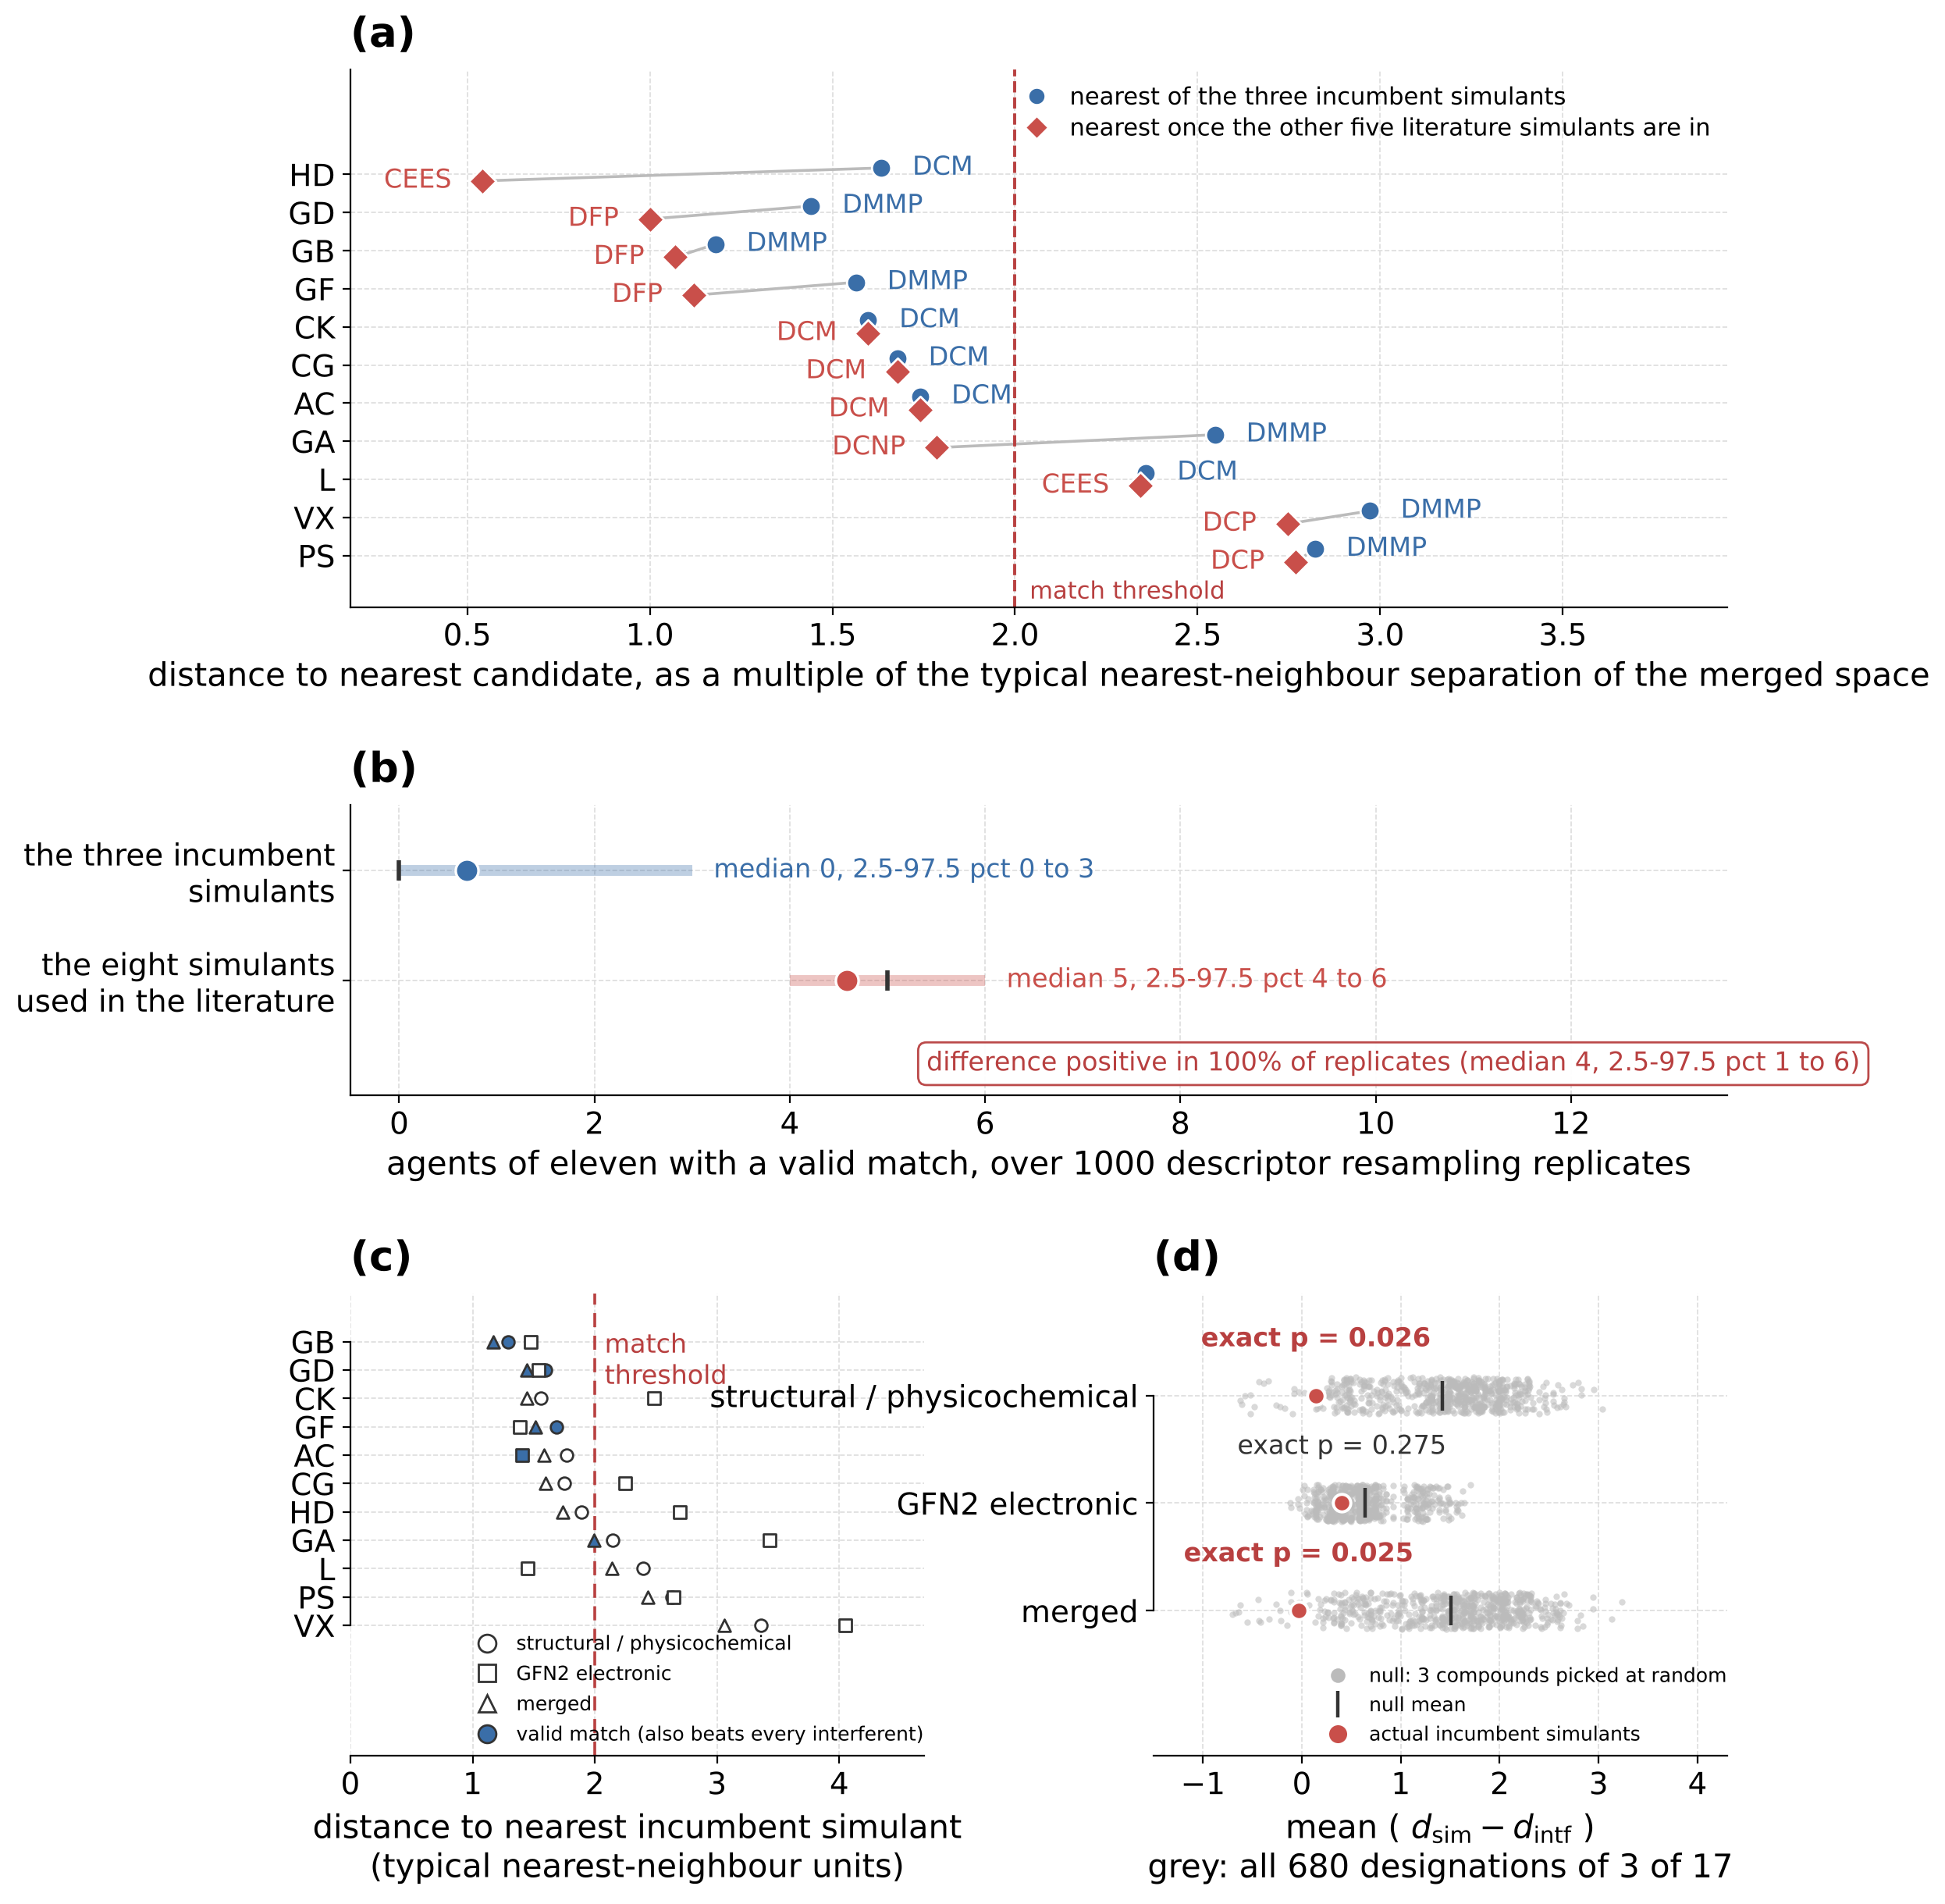
\includegraphics[width=\textwidth]{Fig_main.png}
\caption{What the comparison contains decides the answer. (a) For each agent,
the distance to the nearest incumbent simulant (circles) and to the nearest
candidate once the five further compounds treated as simulants in the
literature are included
(diamonds), as multiples of the typical nearest-neighbour separation of the
merged space on the thirty-five-compound panel. A match requires a normalised
distance below the dashed threshold \emph{and} a distance smaller than that to
every compound not designated a simulant, so sarin, soman and cyclosarin fail on
the primary panel despite lying inside the threshold. (b) Matched agents under
1000 descriptor-resampling replicates (Section~\ref{meth:dboot}) for the
incumbent three and for the eight literature-used simulants examined here;
circles are means, vertical rules medians, bars the 2.5th to 97.5th
percentiles across replicates. (c) On the twenty-eight-compound panel,
which omits those five, the distance from each agent to its nearest incumbent
simulant in each of the three spaces, normalised by the typical
nearest-neighbour separation of that space; filled markers are valid matches.
(d) Exact permutation null for that panel over all 680 ways of designating three
of the seventeen non-agents as simulants, with the actual designation marked;
the $p$ shown is the mean-difference statistic only, the other five and the
adjusted values being in Supplementary Table~\ref{S-tab:ablation}, where the
Benjamini-Hochberg value over its eighteen tests is 0.165.}
\label{fig:main}
\end{figure}

\subsection{What the comparison contains decides the answer}
\label{res:panels}

\begin{figure}[tp]
\centering
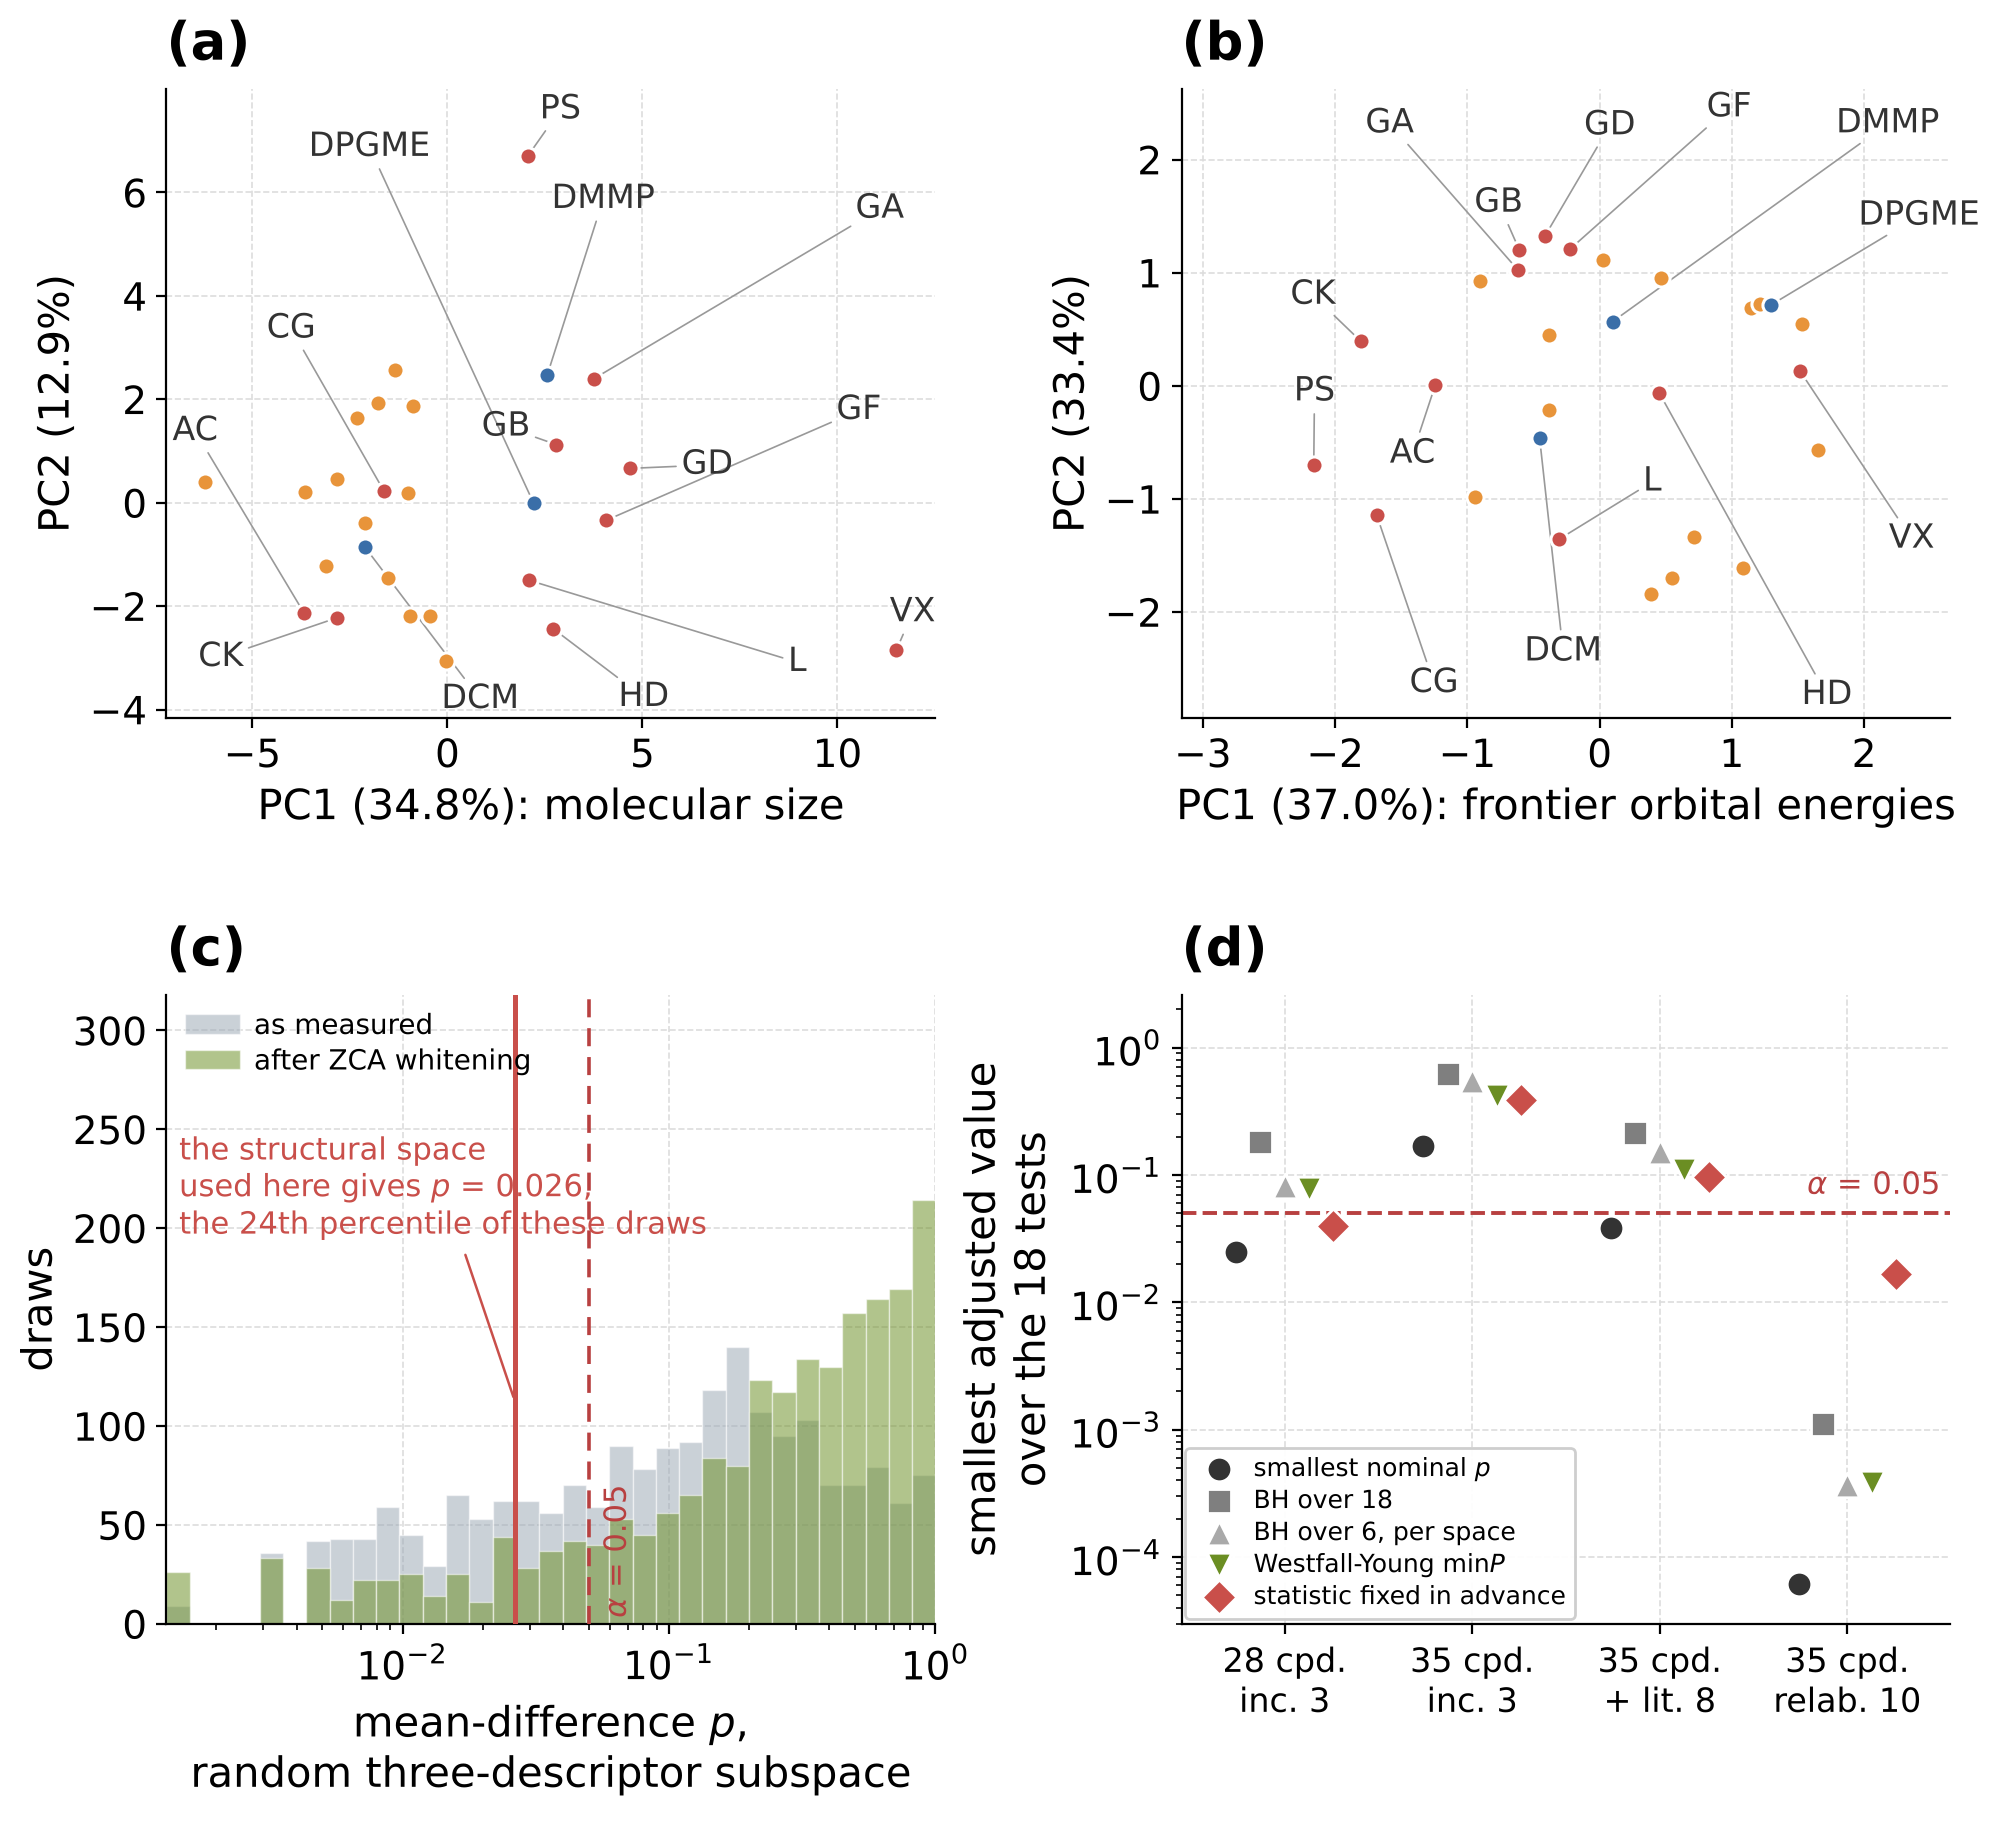
\includegraphics[width=\textwidth]{Fig_spaces.png}
\caption{The spaces the comparison is made in, and what the nominal value is
worth once the choices behind it are counted. Red marks the authentic agents,
blue the three incumbent simulants and orange the interferents and solvents;
only agents and simulants are labelled. (a) Principal components of the
structural space and (b) of the three-coordinate GFN2-xTB electronic space,
both on the twenty-eight-compound panel, so that the five literature simulants
do not appear in them; the
leading structural component is a size axis and the leading electronic component
loads the two orbital energies against the dipole moment. (c) The mean-difference
statistic for 2000 random three-descriptor subspaces of the structural space, before and after ZCA whitening, with the space used here marked: its
0.026 is the 24th percentile of those draws, and 36\% of them fall below 0.05
as measured, 17\% after whitening. (d) Smallest adjusted value over the
eighteen tests of each configuration under the five accounting schemes of
Supplementary Table~\ref{S-tab:family}; on the twenty-eight-compound panel only the
scheme that
fixes the statistic in advance falls below 0.05, and the fourth configuration
falls below it under every scheme. Local reactivity at phosphorus and the rank
of the Parr index are in Supplementary Figure~\ref{S-fig:plocal}.}
\label{fig:spaces}
\end{figure}

On the thirty-five-compound panel, no authentic agent has a valid match to an
incumbent simulant. Figure~\ref{fig:main}a shows why, and the mechanism is not
the one our earlier version reported. The two panels do not share a scale, and
they do not quite share a space. Standardisation and the normalising separation
are recomputed on each panel, and the filters admit different columns on
each, \texttt{kappa1} on the twenty-eight-compound panel against three
phosphorus counts on the primary one, so the structural coordinates are neither
the same set nor the same number, thirty-seven against thirty-nine.
Distances across the two are therefore not directly comparable, and the
comparison we rely on is made within the primary panel, where the compounds,
the columns and the standardisation are fixed and only the labels move. Held on
that single basis, every agent sits exactly as far from its nearest incumbent
whether the designated set is the incumbent three or those three together with
the five literature compounds, because all three incumbents belong to both
sets. The compounds did not become less faithful: on that panel sarin stands
1.18 from DMMP, soman 1.44 and cyclosarin 1.56. What changed is that diisopropyl
fluorophosphate is present, at 1.07, 1.00 and 1.12 from the same three agents,
and the match criterion requires a simulant to be nearer than every compound not
designated one. The same holds across the panel, with 2-chloroethyl ethyl
sulfide at 0.54 from sulfur mustard where dichloromethane stands at 1.67, and
diethyl cyanophosphonate at 1.79 from tabun where DMMP stands at 2.55.
Admitting the five as simulants gives five matched agents of eleven, against
four on the twenty-eight-compound panel and zero on the primary one. The zero
does not depend on the threshold: no incumbent simulant is the
nearest non-agent compound to any of the eleven agents, so the count stays at
zero however far the threshold is relaxed.

That count is sensitive to the descriptors, and the honest statement of it is
the interval rather than the point. Resampling the 42 merged-space descriptors
with replacement (Section~\ref{meth:dboot}) gives the incumbent three a median
of zero matched agents with a 2.5th to 97.5th percentile range of zero to
three, and exactly zero
in 58.6\% of replicates, against a median of five and an interval of four to six
for that eight-compound set, which contains the incumbent three. Because the
match criterion asks whether a designated compound is nearer than every
compound outside the designated set, enlarging that set cannot lower the count,
and part of the difference is set size alone: designating eight non-agents at
random matches 2.68 agents on average against 1.00 for three, so the observed
gap of five decomposes into 1.68 expected from size and 3.32 beyond it. Matching
on size alone is not quite the right null, because the observed eight-compound
set contains the incumbent three while a set drawn freely need not. Holding the
three fixed and drawing the other five at random gives a mean of 1.92 rather
than 2.68, and the observed five sits at $p=0.068$ against it. Neither observed
count departs from a null built to resemble it: the three at $p=0.479$ over all
2024 designations, and the eight at $p=0.068$ conditionally or $p=0.161$
unconditionally. We report the lower tail for the three because the observed
count is zero, which is the floor; the upper tail there is 1.000 by arithmetic
and says nothing, and an earlier version of this paper quoted it as though it
did. The lower tail carries its own limit, and it belongs here rather than in a
footnote: because zero is the smallest count attainable, $p=0.479$ is the
smallest lower-tail value this comparison can ever return. It does not report a
result that failed to reach significance. It reports a comparison that cannot
reach significance at any conventional level, whatever the data. What the resampling adds is that the
difference between the counts, unadjusted for size, is positive in 1000 of 1000 replicates, median
four, interval one to five (Figure~\ref{fig:main}b). The per-agent reliabilities
in the same replicates separate the firm results from the marginal ones. Sulfur
mustard is matched by 2-chloroethyl ethyl sulfide in every replicate and tabun by
diethyl cyanophosphonate in 51.2\%, while under the incumbent set alone sarin
recovers DMMP as its nearest compound in 38.0\% of replicates, soman in 14.9\%
and cyclosarin in 11.4\%. The displacement of DMMP at the G agents is therefore
the weakest part of the picture and the sulfur mustard result the strongest,
reversing what the point estimates suggest.

Figure~\ref{fig:spaces}a and b give the spaces on the twenty-eight-compound
panel. The leading structural component is a
size axis carrying 34.9\% of the variance and the leading electronic component
loads on the two orbital energies against the dipole moment, the first two
carrying 70.4\%. The primary panel behaves the same way, at 34.9\% and 70.3\%.
Merging the two blocks returns a size axis at lower cumulative variance over the
first two components, 45.7\% on the smaller panel and 45.2\% on the primary one,
for a dimensional rather than a chemical reason: at equal
per-descriptor weighting the structural descriptors, thirty-seven on the smaller
panel and thirty-nine on the primary one, outvote three electronic ones.

Every exact permutation test we can run, across four panel and designation
configurations, three spaces and six statistics, is in Supplementary
Table~\ref{S-tab:ablation}, in full rather than selected from, because the
pattern across the cells is the finding. Three things hold across it. On the
primary panel no test reaches nominal significance: in no space and under no
statistic are the incumbent simulants distinguishable from compounds drawn at
random. Classing the five literature compounds as simulants recovers two
nominal values below 0.05, both in spaces containing the structural
descriptors, so the difficulty is not that the test cannot detect anything on
this panel. On the twenty-eight-compound panel, which differs only in omitting
those five and two organophosphorus pesticides, the incumbents beat random
compounds under two of six statistics in the structural space and three of six
in the merged space.

Correcting for the number of times we looked removes almost all of it, and the
exception is instructive. On the primary panel the question does not arise,
since the smallest nominal value is already 0.156 under the per-descriptor
standardisation used throughout. The five accounting schemes of Supplementary
Section~\ref{S-meth:multiplicity}, applied in Supplementary
Table~\ref{S-tab:family}, matter only for the twenty-eight-compound panel. There the eighteen-test family
gives a smallest adjusted value of 0.181, correcting the six statistics within
each space gives 0.074, and the Westfall-Young min-$P$ procedure, which uses the
shared permutations and so accounts for the dependence between the tests exactly
rather than approximating it, gives 0.078. That is the closest any correction
brings the panel to the conventional threshold without crossing it. The fifth
scheme behaves differently. Had the mean difference been specified in advance as
the single statistic, three tests would have been run and the
twenty-eight-compound structural and merged results would survive at $q=0.040$,
while neither thirty-five-compound configuration would (0.386 and 0.092). We did
not specify a statistic in advance; we computed six and chose among them after
seeing them, which is the circumstance the correction is for. The comparison is
the paper's own argument made with its own data: one analysis, one data set,
five defensible ways of accounting for the search, and a result significant under
one and not the other four. The declaration that would have made the difference
is one nobody in this literature makes, and it has to be made before the data
are seen.

One label decision carries more than any of this. Section~\ref{meth:panels}
classes dichlorvos and malathion as interferents and records that decision as
contestable. Classing them as simulants instead, which moves two labels and
changes nothing else, gives a smallest nominal value of 0.00006 and a
Benjamini-Hochberg value of 0.0011 over the same eighteen tests, and it is the
only configuration in this work that survives every one of the five accounting
schemes of Supplementary Table~\ref{S-tab:family}. The direction is
not surprising, since both pesticides carry the phosphoryl motif the agents
carry, and that is the point: significance here is available to an analyst who
moves two labels, and the practice records neither which labels were moved nor
that any were. This is not a recommendation, and the reason it is not is
narrower than we first wrote. We described the two pesticides as compounds
nobody uses as simulants. That is wrong for one of them: the NIOSH document
cited throughout this section lists malathion in its GB simulant column and
reports breakthrough times for it through protective clothing materials
\cite{niosh2002simulant}. Dichlorvos we still find in no such role. So the
relabelling that produces the only result surviving every accounting scheme is
not an arbitrary one, which strengthens rather than weakens the point: a
defensible label change, made by an analyst with a citation in hand, moves this
analysis from nothing at $q=0.617$ to $q=0.0012$, and the practice records
neither that a label was moved nor which one. What the comparison shows is that
a designated set can be made to look supported by choosing what goes into it.

One further observation bounds what the nominal values can mean. The count of
agents for which a compound outside the designated set is nearer than any
incumbent simulant is 11 of 11 in the merged space of the primary panel against
a null expectation of 9.63 set by the 21:3 group-size asymmetry alone, and 6, 10
and 6 of 11 in the three spaces of the smaller panel against 9.06, so the raw
count carries no evidence without the permutation test and in one space runs the
wrong way.

The difference between the two spaces is chemical rather than geometric.
Truncating the standardised structural space to its first three principal
components strengthens the result rather than weakening it, from $p=0.026$ to
$p=0.0029$ on the twenty-eight-compound panel, which leaves the two spaces
94-fold apart in $p$ at matched dimension. What the nominal structural value is
worth against the descriptors it was drawn from is a separate question, and
there the answer has two parts that point in opposite directions, and an earlier
version of this paper reported only the first. Of 2000 random three-descriptor
subsets of that space, the observed 36-dimensional value of 0.026 sits at the
24.3rd percentile of the resulting distribution while the electronic value of
0.275 sits at the 75.5th: the full-space value is an ordinary draw among the
descriptor subsets we could have used instead, which is a statement about
descriptor choice and is the one we rely on.

The second part is that 36.0\% of those subsets reach $p<0.05$, and we first
read that as showing the same thing. It does not. In a fixed subspace the
permutation $p$ is the rank of the designated set among all 680 designations, so
if the designation were arbitrary the expected share below 0.05 would be 0.05.
We therefore recomputed the share for every one of the 680 designations over the
same subspaces (Section~\ref{S-res:subspacenull}). The mean is 4.7\%, as it
should be; the incumbent designation's 36.0\% ranks fifth of 680, $p=0.0074$.
The structural block therefore does carry something that distinguishes the
incumbents from an arbitrary triple, and we withdraw the claim that this control
shows otherwise.

What it carries is narrower than it sounds, and the sign of the statistic says
so. The observed mean difference in the structural space is $+0.155$: the
designated simulants are on average \emph{further} from the agents than the
nearest compound outside the designated set. What the test detects is that they
are less far than a triple drawn at random from a pool assembled out of
interferents and solvents, which were chosen for this panel because they are not
like the agents. Against that reference class a single organophosphorus compound
is close to sufficient. Supplementary Section~\ref{S-res:dimdetail} reports
both controls in full.

\subsection{How many agents have a valid simulant depends on the panel}
\label{res:match}

Table~\ref{tab:match} lists, for each agent on the twenty-eight-compound panel,
the nearest incumbent simulant in the merged space as a multiple of that space's
typical nearest-neighbour separation. Sarin (1.171), soman (1.445),
cyclosarin (1.449) and tabun (1.905) are matched, all four by DMMP; VX at
2.922 is not. Tabun clears the threshold of 2 by 0.095, and we flag that rather
than report it as a result: an earlier version of this analysis, which retained
a structural coordinate that is an exact function of two others
(Section~\ref{meth:descriptors}), put tabun at 2.003 and counted three matches
here instead of four. A count that moves when a redundant coordinate is removed
is a count that should be read as marginal, which is the same lesson the rest of
this paper draws about the panel. DPGME is nominally VX's nearest simulant in all three spaces, but
at 3.060 typical separations in the merged space and 3.357 in the structural
space that is not a match in any useful sense. Dichloromethane, which the
sensor literature we surveyed runs against the whole panel rather than against a
named agent \cite{lee2011sno2}, is not phosgene's nearest neighbour in any of the
three spaces: ethyl acetate leads it in the structural space (1.136 typical
separations against 1.750) and in the merged space (1.120 against 1.600), and
chloroform in the electronic space (1.171 against 2.247).

The direction of the comparison matters. Table~\ref{tab:match} gives, for each
agent, its nearest simulant; the reverse question is which agent each simulant
is nearest to, and over the same 1000 descriptor-resampling replicates of
Section~\ref{meth:dboot} the three incumbents separate. DMMP is nearest sarin in
92.8\% of replicates and nearest one of the four G-series agents in 99.5\%.
Dichloromethane is nearest a G-series agent in 4.2\%, sitting instead with the
choking and blood agents. DPGME divides evenly, sulfur mustard in 38.2\% and the
G series in 56.9\%. Being nearest is not being close, and DPGME carries no valid
match in any space on this panel; but it is the one of the three whose
designating document names a class, ``a preferred G agent simulant''
\cite{seitzinger2006simulant}, and it is the one whose class these spaces do not
resolve.

\begin{table}[!htb]
\centering
\caption{Nearest incumbent simulant for each agent on the twenty-eight-compound
panel, as a multiple of the typical nearest-neighbour distance of the merged
space. A match requires a normalised distance $\le 2$ together with a distance
smaller than that to every compound outside the designated set. On the primary
thirty-five-compound panel no agent has a match.}
\label{tab:match}
\small
\begin{tabular}{llcc}
\hline
Authentic agent & Nearest simulant & Normalised distance & Valid match \\
\hline
GB & DMMP & 1.171 & yes \\
GD & DMMP & 1.445 & yes \\
CK & DCM & 1.446 & no \\
GF & DMMP & 1.517 & yes \\
AC & DCM & 1.587 & no \\
CG & DCM & 1.600 & no \\
HD & DCM & 1.740 & no \\
GA & DMMP & 1.995 & yes \\
L & DCM & 2.141 & no \\
PS & DMMP & 2.433 & no \\
VX & DPGME & 3.060 & no \\
\hline
\end{tabular}
\end{table}

The count is stable but not invariant, and the two spaces admit tabun at
different bars. In the merged space the set is \{GB, GD, GF\} at thresholds of
1.5 and 1.75 and \{GB, GD, GA, GF\} at 2.0, 2.5 and 3.0, tabun entering once the
bar passes its value of 1.995. In the structural space it is \{GB\} alone at 1.5,
with soman at 1.600 and cyclosarin at 1.687 outside, \{GB, GD, GF\} at 1.75 and
2.0, and four only at 2.5. The four-agent figure is therefore a statement about
the merged space at a threshold of exactly 2.0, and the three-agent figure the
same space one notch lower. The electronic
space is the exception, and it is the informative one: there the count is one at
every threshold tested, hydrogen cyanide matched by dichloromethane at 1.407,
because acetonitrile sits closer to sarin, soman and cyclosarin than DMMP does
and all three fail the threshold-free condition outright. Over the thresholds
tested the count does not exceed four of eleven in any space.

The dependence on the panel is sharper than the dependence on the threshold. On
the thirty-five-compound panel, with the incumbent three still the only
simulants and the five literature compounds in the comparison pool, the merged
space returns no valid match for any of the eleven agents: DMMP loses GB, GD and
GF to diisopropyl fluorophosphate, which is nearer to all three. Admitting the
five as simulants gives five matches of eleven, more than the incumbent set
achieves on either panel, with DFP taking sarin, soman and cyclosarin at 1.06,
0.99 and 1.11, diethyl cyanophosphonate taking tabun at 1.79, and
2-chloroethyl ethyl sulfide taking sulfur mustard at 0.57, the closest
agent-simulant pair anywhere in this work. VX remains unmatched in every panel
and space we examined.

We draw no conclusion from this that the field should switch compounds, because
the five were not selected by any procedure we can inspect either, and
Section~\ref{res:panels} applies to them exactly as it applies to the incumbent
three. What the comparison establishes is narrower: the statement ``three of
eleven agents have a valid simulant'' is true of one panel, false of a second,
and replaced by a different list on a third, which is the same instability the
permutation tests report and not an independent finding.

One agent deserves a note of its own. Lewisite's incumbent simulant is
dichloromethane, which shares neither its central element nor its halogen
count, so the failure might be read as an artefact of that comparator rather
than of the designation. Arsenic trichloride, used as a lewisite
simulant in the sensing literature \cite{lee2016lewisite}, though we found
no designating document for it, leaves the incumbent-three count at zero of
eleven and supplies lewisite's only match under the literature set, at 1.25
where the best the five could previously offer was 2-chloroethyl ethyl
sulfide at 2.35 (Supplementary Information).

\subsection{What the array actually measures}
\label{res:measured}

Every argument above rests on descriptor distances, and the premise that one of
those spaces corresponds to what a vapour-phase sensor reports is tested in
Supplementary Section~\ref{S-res:arraydetail} against measured colorimetric
response for twelve panel compounds over 29 dyes, of which 23 are independent
channels in the one plate set where that matters. It does not resolve the
question, and it is worth being exact about why. Of twelve
panel-channel-space cells, three reach a nominal
$p<0.05$ under Mantel permutation over compounds and they do not agree on a
space; corrected across the twelve, the
smallest adjusted value is 0.100 and no cell reaches $q<0.05$. All three of
those cells lie in the plate set that contains no simulant, so they compare one
agent with another and not a simulant with an agent. The six cells that bear on
the premise are the six in the set that holds DMMP, and all six are null.
Simulating the test actually run, the exact Mantel over all 720 relabellings of
six compounds, the design detects $|\rho| \ge 0.67$ at 80\% power, so these data
exclude a strong association and nothing weaker. The premise is therefore
untested rather than supported, and every distance-based claim in this paper
inherits that. Three artifacts are
reported there because our own
first version contained all three: dye-axis centring fixes the between-compound
mean cosine at $-1/(n-1)$, which the observed means clear by only 0.013 to
0.064; six dyes that do not fluoresce under ultraviolet illumination returned
one background reading six times, which we now collapse; and the measured agent
nearest to DMMP in the ultraviolet channel is tabun rather than sarin, which the
descriptor criterion of Section~\ref{res:match} excludes.

\subsection{The toxicity half of the criterion}
\label{res:toxsummary}

\begin{figure}[tp]
\centering
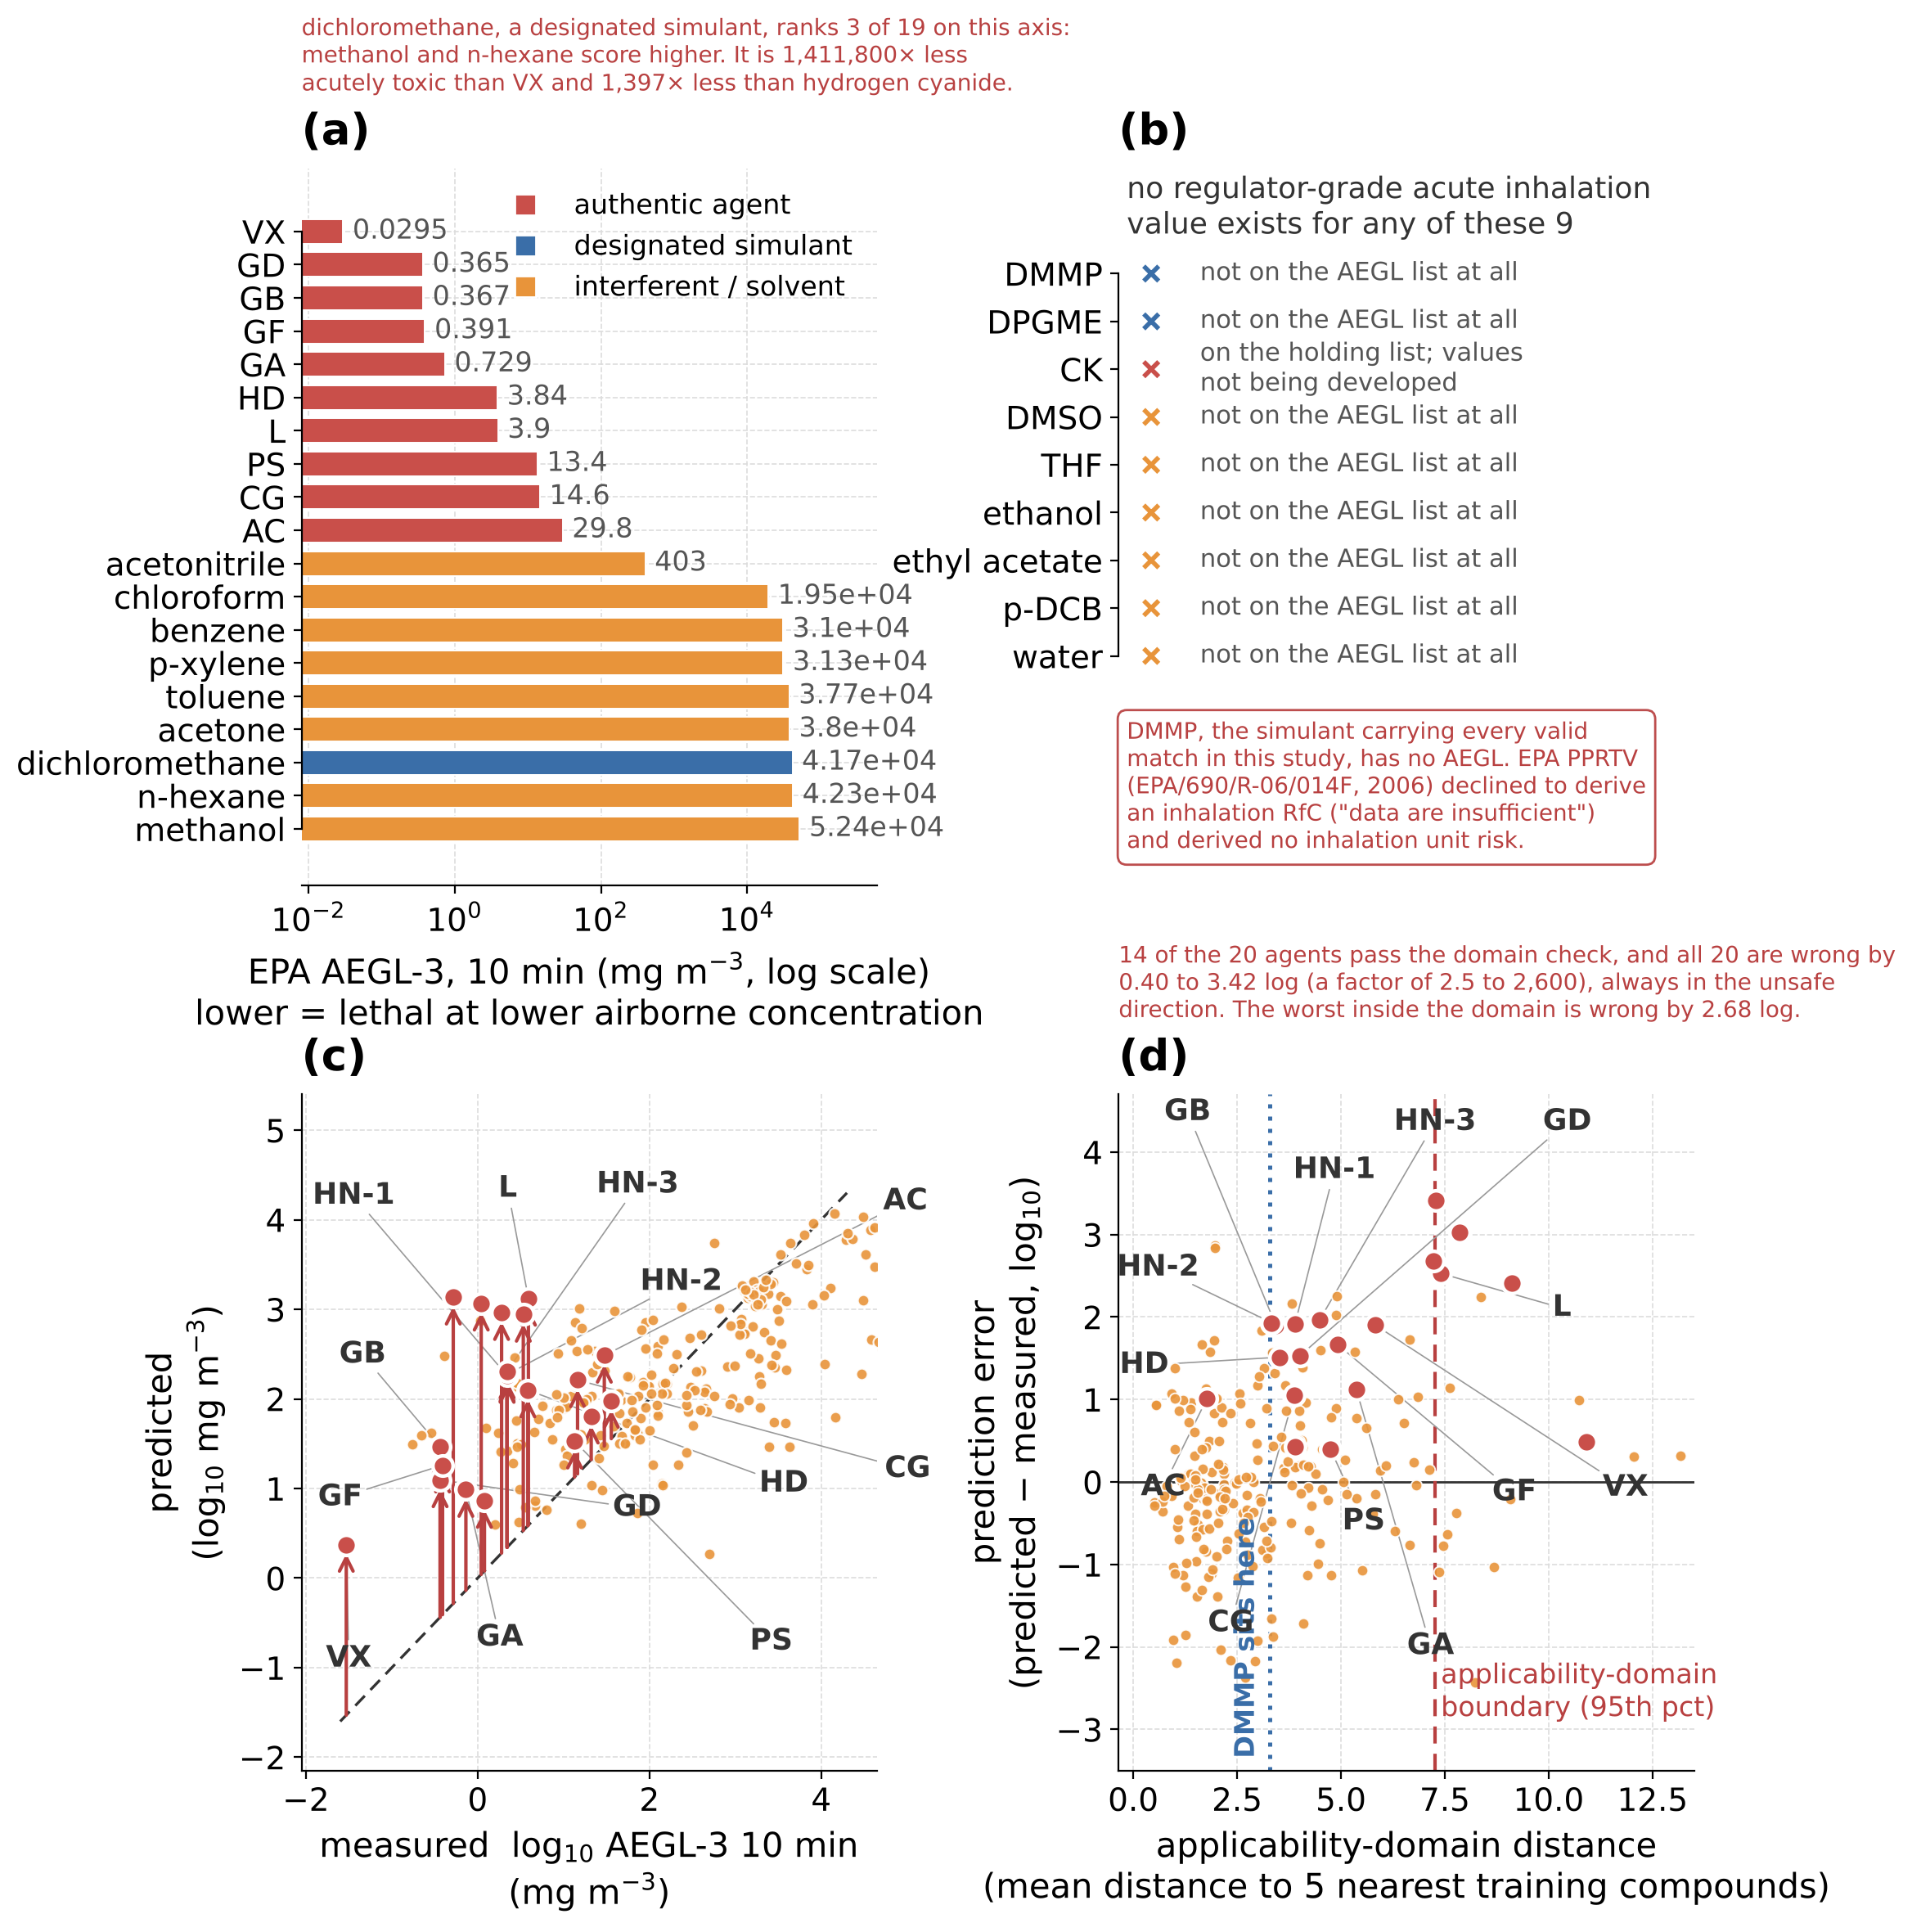
\includegraphics[width=\textwidth]{Fig_toxicity.png}
\caption{The second half of the criterion, measured and then modelled.
(a) EPA AEGL-3 at 10~min on a logarithmic scale for the nineteen compounds that
have one; the incumbent simulant dichloromethane sits near the safe end but is
not the safest, methanol and n-hexane both scoring higher.
Five of the nineteen values come from the agency's own footnotes rather than
from the table cell, because they exceed half the lower explosive limit.
(b) The nine compounds with no regulator-grade acute inhalation value, with the
reason for each; DMMP, which supplies every valid match on the
twenty-eight-compound panel and zero on the primary one, is among them.
(c) Out-of-fold predictions for the 230 training chemicals (orange) with the
twenty military agents held out of training (red) overlaid; arrows run from the
measured
value to the prediction, and every agent is predicted safer than it is. Labels
name the ten agents of this paper's panel that the AEGL set also holds and the
three nitrogen mustards; the remaining seven held-out agents are plotted
unlabelled. (d) Prediction error against
applicability-domain distance. Every one of the twenty is wrong by between 0.40
and 3.42 log units, and fourteen of them pass the domain check, the
worst of those fourteen being wrong by 2.68 log units. The dotted line marks
where DMMP sits.}
\label{fig:tox}
\end{figure}


The criterion has a second half: that compounds chosen on physicochemical
grounds present minimal toxicity risk \cite{webb2025}. We tested it on the same
panel and report it in full in the Supplementary Material. Three results are
needed here.

Dichloromethane has a regulator-derived acute inhalation value and DMMP has
neither an acute one nor a chronic one: it is absent from the AEGL list, and
EPA's provisional assessment separately declined to derive a chronic inhalation
reference concentration for want of data (Figure~\ref{fig:tox}a and b,
Supplementary Section~\ref{S-meth:aegl}). The two incumbents
therefore differ in how well documented they are and not only in how hazardous,
which matters because DMMP is also the compound against which decontamination
efficiency is quantified \cite{ebeam}. Dichloromethane's value is favourable on
the acute axis, at the 96th percentile of a 207-compound pool, and
says nothing about the chronic and carcinogenic classification now displacing it
from solvent inventories.

A model cannot fill the gap. A random forest trained on 230 AEGL chemicals
reaches $R^{2}=0.458$ and then predicts every one of twenty held-out military
agents safer than measured, by factors of 2.5 to 2600, while certifying fourteen
of them as inside its applicability domain (Figure~\ref{fig:tox}c and d,
Supplementary Section~\ref{S-sec:qsar}). The failure is not a missing mechanism, since
thirteen training compounds carry an acetylcholinesterase-inhibiting
pharmacophore and one is more acutely toxic than sarin. It is tail regression, a bias in
the response space that an input-space domain check cannot see.

Fidelity and acute toxicity show no monotonic association across the 207
compounds carrying both measured axes (Spearman $r=+0.062$, 95\% CI $-0.077$ to
$+0.199$). The interval excludes a trade-off strong enough to constrain
selection, which is weaker than independence and is what the data support, so
the two can be improved separately
(Supplementary Section~\ref{S-res:h1}). We draw no candidate recommendation from
that: one resting on a single panel and two axes would repeat the error this
paper reports.

\section{Discussion}

The criterion by which low-toxicity simulants are chosen is stated clearly
enough to test \cite{webb2025}: align hydrophobicity, volatility and solubility
with the agent. What the practice does not state is what the chosen compounds
should be compared against, and that decides the answer. On a panel containing
the compounds the field itself uses as simulants, the three incumbents match no
agent and no test reaches nominal significance; on a panel omitting them, four
agents are matched and the smallest nominal value is 0.025.

The mechanism is not a story about fidelity. The incumbents sit almost as close
to the agents on one panel as on the other, and on a single standardisation
basis they do not move at all (Section~\ref{res:panels}). What the larger panel supplies is
diisopropyl fluorophosphate, nearer to sarin, soman and cyclosarin than DMMP is,
so a criterion that asks a simulant to beat the alternatives returns nothing.
Resampling the descriptors leaves the aggregate comparison intact in every
replicate, but not each displacement within it: sulfur mustard is matched by
2-chloroethyl ethyl sulfide in all of them while the incumbent set recovers DMMP
at sarin in 41.0\%, soman in 14.4\% and cyclosarin in 11.4\%, so the G-series
displacement is the weakest part of this and the mustard result the strongest. A designation
defended by a comparison that excludes the alternatives is not defended.

An earlier version of this work reported the twenty-eight-compound structural
cell as the finding and built a thesis on the contrast between it
and the electronic space. Three things undo that reading, and each is a mistake
another group could make the same way. The value does not survive the eighteen
tests of its own family (Benjamini-Hochberg $q = 0.181$), although it would have
survived at $q = 0.040$ had the statistic been fixed in advance, which
demonstrates the paper's argument rather than defending the value. It sits at the
24.3rd percentile of 2000 arbitrary three-descriptor slices of the same block,
so the particular space we used is not what produced it. And it is specific to
the panel that omits the five. What does not undo the reading, and what we
reported as though it did, is the share of those slices reaching $p<0.05$:
corrected against the 680 designations that share generates, the incumbent
designation ranks fifth (Section~\ref{res:panels}).

Two things we expected to dissolve the contrast between the spaces did not. The
Parr electrophilicity index was an exact function of two of the other electronic
descriptors, so the electronic space never had the dimension we reported;
removing it moved that space's value only from 0.297 to 0.275. Matching the
dimensions did not dissolve the contrast either (Section~\ref{res:panels}). What
does weaken it is the choice of electronic-structure method. Rebuilding the
electronic space from density-functional orbital energies moves it from 0.275 to
0.128 and from one valid match to four, three of them the agent and simulant
pairings the sensor literature asserts (Section~\ref{S-meth:dft}). We therefore withdraw the
contrast as something to build on: it is not a stable feature of the comparison,
and the structural value anchoring it is in any case an ordinary draw from the
subspaces we could have chosen.

What remains is a claim about comparison rather than about chemistry. On the
primary panel we cannot establish that the incumbent simulants are closer to the
agents than compounds drawn at random, and we cannot establish the opposite
either. What we can establish is that the compounds which would make the
comparison informative were not in it.

The documentary record explains how that arose, and it is not a story about
carelessness. Two of the three were designated carefully for measurements that
are not the one they are now asked to support (Section~\ref{res:docs}): DMMP
for adsorptive breakthrough on a filter bed \cite{niosh2002simulant}, DPGME for
ion-mobility detectability in a training composition
\cite{seitzinger2006simulant}. Each selection was fit for its own measurement.
The compounds then carried their status into sensor development, where the
governing property is the response of a dye or an electrode rather than a
breakthrough time, and nothing in the original validation speaks to that. For
dichloromethane we found no designating document at all.

The absence this paper documents is specific rather than general. A
safety-screened repository of candidate simulants exists \cite{james2021}, and a
descriptor-based selection procedure appeared in this journal fifteen years ago
\cite{lavoie2011}. What is missing is any route by which either reached the
compounds the detection literature settled on.

That mechanism is general. A simulant is validated against a measurement rather
than against an agent, and treating the validation as a property of the compound,
so that it travels into a new application, produces a working set whose standing
no descriptor space can reproduce. The corrective is not a replacement compound
but a declaration: which measurement a simulant was validated against, and a
panel, space and statistic fixed before a claim that it is valid for a different
one is tested. Agrawal et al.~\cite{agrawal2018} reach the same place from the
other direction, adequacy being a property of the compound together with the
measurement it stands in for.

Three consequences follow for practice. DMMP is a surrogate for one G agent at a
time rather than for the G series, and not a V-agent surrogate at all: the
descriptor criterion assigns GB, GD and GF to it, while the measured array puts
sarin first in reflectance and tabun, which fails that criterion, first in the
ultraviolet channel (Supplementary Section~\ref{S-res:arraydetail}). The
condensed Fukui index at phosphorus puts DMMP above VX by a factor of 2.7 in the
semi-empirical treatment used here, which would sharpen the point, but we could
not reproduce that index at a higher level of theory and we do not lean on it
(Supplementary Section~\ref{S-meth:dft}). The global electrophilicity index
should not enter a descriptor space, for an arithmetic rather than a chemical
reason: where the frontier orbital energies are present it adds no information,
and a correlation filter will not notice. It should not be read as a reactivity
axis either, and that is a chemical reason: recomputing this panel with density
functional theory leaves the qualitative picture but moves which agents sit
lowest, so an ordering taken from it describes the method
(Supplementary Section~\ref{S-res:plocal}). And
the safety of a simulant is a question about evidence before it is one about
hazard, since dichloromethane carries a regulator-derived acute inhalation value
and DMMP carries none (Section~\ref{res:toxsummary}).

We did not attempt to improve the toxicity model by training on organophosphorus
compounds, and the distinction is narrower than a refusal to model the
chemistry. Mechanistic structure--activity models of organophosphorus lethality
exist and we have contributed to them \cite{qsarld50}; such a model assesses
compounds that already exist. What we decline to build is the same instrument
turned into a design objective, a predictor of mammalian lethality evaluated
over structures not yet made inside a loop that proposes them, which is the
configuration in which a safety model becomes a potency model
\cite{urbina2022}. The cost is an acknowledged gap: for the compound class of
greatest interest we can say that a predicted value is unreliable and cannot
supply a better one. Reporting the gap rather than closing it is the correct
outcome, and where to set that boundary is contested rather than settled
\cite{cbrndisclose}.

\paragraph{Limitations.} The documentary findings of
Section~\ref{res:docs} rest on public sources, and the scope of that search
is stated there. The claim is that no public instrument designates these three
compounds for the use the sensor literature makes of them, not that no
instrument does. A null result invites the question whether the design could have seen an
effect. On the primary panel the mean-difference statistic reaches $p<0.05$ once
the incumbent simulants are moved 0.22 typical nearest-neighbour separations
closer to the agents, while the deficit they actually carry has a median of
0.445 and falls below that value only at sarin, where it is 0.110
(Supplementary Section~\ref{S-res:mde}). The test is therefore sensitive to effects
smaller than the one at issue. The
agent set is eleven compounds and the nearest-neighbour statistics inherit that:
on the larger panel with eight simulants, leaving out one agent at a time moves
the structural $p$ between 0.020 and 0.186, the worst case being removal of
tabun, so a result one of eleven agents can carry across the 0.05 line is not a
property of the panel. The
permutation test is directional and reported one-sided, with both two-sided
conventions given in Section~\ref{sec:perm}. The two panels are the two we could
build from compounds carrying complete descriptor data; measured toxicity values
exist for a subset only, DMMP among the compounds without one, so the two axes do
not run over the same compounds. A fourth configuration,
classing dichlorvos and malathion as simulants, is reported in
Supplementary Table~\ref{S-tab:ablation} and Section~\ref{res:panels} because we
flagged that
label decision as contestable; the four configurations sample the configuration
space rather than census it. Accordingly, the present panels should be
interpreted as demonstrations of panel dependence rather than as exhaustive
representations of all compounds that have been used as chemical warfare agent
simulants. One omission is worth naming because it is systematic. Probe
chemistries for lewisite are developed against arsenic trichloride
\cite{lee2016lewisite}, which is in neither panel, and the structural filter of
Section~\ref{meth:filter} flags every arsenical, so a compound of that class
could not have been admitted as a candidate in the toxicity screen either. The
arsenical route to a lewisite simulant is therefore outside what is tested
here, and lewisite's lack of a valid match in any space should be read against
that. The measured-array intervals describe variation across concentrations within
one plate set rather than agreement between preparations (Supplementary
Section~\ref{S-res:arraydetail}). GFN2-xTB is
semi-empirical, and the quantities used here are relative within a consistent
protocol rather than absolute. The virtual orbital energies make that concrete.
Across the thirty-five-compound panel they run from $-9.64$~eV for chloropicrin
to $+2.23$~eV for water, and twenty-four of the thirty-five fall below
$-4$~eV. Read as electron affinities in the Koopmans sense those values are not
attainable, chlorine being the most electron-avid element at 3.6~eV, so the
method's virtual eigenvalues are coordinates and not affinity estimates. Every
distance reported here is computed on descriptors standardised within the panel,
which leaves a shift and a scale applied to a whole axis without effect. What
such an axis cannot carry is a claim about any one compound's absolute frontier
energy, and we make none.

\section{Conclusions}

Simulant validity cannot be treated as an intrinsic property of a compound. It
depends on the measurement it is intended to reproduce and on the comparison
against which that claim is evaluated, and the practice of choosing chemical
warfare agent simulants records neither. On a panel of
thirty-five compounds that includes the five the sensor, sorbent and
decontamination literature also uses as simulants, not one of eleven authentic
agents has a valid match to an incumbent simulant and not one of eighteen tests
reaches nominal significance. The incumbents are no further from the agents on that
panel than on the smaller one; diisopropyl fluorophosphate is simply nearer, and
under descriptor resampling the incumbent three match a median of zero agents
against five for the eight literature-used simulants examined here, the
difference positive in every
one of 1000 replicates. Omitting those five restores four matches and a nominal
structural $p$ of 0.026, a value at the 25.9th percentile of 2000 arbitrary
three-descriptor subspaces of the same block which no correction over the
eighteen tests run leaves significant.

The documentary record gives the reason. DMMP was designated for filtration
breakthrough testing and DPGME for ion-mobility training compositions, neither
of which is detection chemistry; for dichloromethane we found no designating
instrument at all. A simulant is validated against a measurement, and that
validation does not travel with the compound into a new application.

The absence of evidence is not evidence of unsuitability, and we draw no
conclusion that the incumbents are poor choices. What we conclude is narrower
and addressed to method. A simulant claim is testable, this field has
the data to test it, and the test returns whatever the analyst's undeclared
choices imply. Moving two labels, from interferent to simulant, is enough to
turn a result that survives no correction into one with an adjusted value of
0.0011. The practical form of that conclusion is a reporting rule: a
simulant result should name the measurement the compound was validated against
and the comparison set it was tested in, and should fix the panel, the
descriptor space, the statistic and the descriptor weighting before the test is
run, and should state how any conformer-dependent descriptor was taken. We add
the last of those because we had not counted it ourselves until a reproduction
check found it (Section~\ref{S-meth:conformer}); unlike the other four it does
not move the answer here, but nothing in the design guaranteed that. Until those are declared in
advance, a statement that a compound is a validated simulant reports a convention
rather than a measurement.

Findings from the toxicity axis are in the Supplementary Material and do not
depend on the contested comparison. The two incumbents differ in how well
documented they are and not only in how hazardous, dichloromethane carrying a
regulator-derived acute inhalation value and DMMP carrying none of any kind
(Section~\ref{res:toxsummary}). A random forest trained
on 230 AEGL chemicals predicts all twenty held-out military agents safer than
measured, by factors of 2.5 to 2600, so predicted toxicity cannot stand in for
the missing values (Supplementary Section~\ref{S-res:qsar}). Fidelity and acute
toxicity show no monotonic association across the 207 compounds carrying both axes
(Supplementary Section~\ref{S-res:h1}). We propose no replacement compound,
because proposing one would repeat the error this paper is about.

\section*{Funding}
This research did not receive any specific grant from funding agencies in the
public, commercial, or not-for-profit sectors.

\section*{CRediT authorship contribution statement}
\textbf{Ku Kang:} conceptualisation, methodology, software, formal analysis,
investigation, data curation, visualisation, writing -- original draft.
\textbf{Jin Yoo:} methodology, investigation, validation, writing -- original
draft. \textbf{Jeongyun Kim:} formal analysis, investigation, validation.
\textbf{Miae Kim:} investigation, validation, writing -- review and
editing.
\textbf{Doo-Hee Lee:} validation, resources, writing -- review and
editing, supervision. \textbf{Yoon Jeong Jang:} validation, writing -- review
and editing, supervision, project administration. Ku Kang and Jin Yoo
contributed equally. Doo-Hee Lee and Yoon Jeong Jang are joint corresponding
authors.

\section*{Declaration of competing interest}
The authors declare no competing financial interest.

\section*{Declaration of generative AI and AI-assisted technologies}
During the preparation of this work the authors used a large language model
(Anthropic Claude) to assist in drafting and editing prose, in writing and
auditing the analysis and figure scripts, and in building the
internal-consistency checks described under Reproducibility. No numerical
result was produced by the model: every value reported here is read from the
output of the deposited scripts, which were executed to generate it. The
authors reviewed and edited all content and take full responsibility for it.

\section*{Data and code availability}
Descriptor tables, parsed AEGL values with their sources, permutation
distributions, candidate tables and all analysis and figure scripts are in a
public repository at
\url{https://github.com/bisu9082/simulant-designation-evidence}, at the tagged
release \texttt{v1.0}, and are also provided with this article. The repository
also carries the primary EPA source document from which every toxicity value
here was parsed, so the parse can be checked against the original. The exact
permutation test is exhaustive and the remaining analyses are deterministic
given the stated seed. The descriptor cache is checked against the code rather
than taken on trust: \texttt{build\_descriptors.py --verify} rebuilds every
numeric column and the analysis pipeline stops if any column fails to
reproduce. Section~\ref{S-meth:conformer} reports what that check caught.

\bibliography{refs}

\end{document}
